\chapter{Referencial Teórico}
\label{chap:3}

\section{Modelos Estatísticos}

Começamos esta seção descrevendo os principais modelos estatísticos utilizados para gerar dados sintéticos para o EJ. A utilização de modelos adequados é importante para gerar dados fidedignos em que conhecemos o resultado correto para que possamos exercitar os modelos de classificação utilizados no EJ e compará-los com a realidade conhecida.

\subsection{Distribuição Beta}

A distribuição beta é uma família de distribuições bastante flexivel e é muito utilizada para modelar experimentos aleatórios cujas variáveis assumem valores no intervalo $(0,1)$, dada a grande flexibilidade de ajuste que seus parâmetros proporcionam. Uma variável aleatória contínua $Y$ tem distribuição beta com parâmetros $\alpha_1 > 0$ e $\alpha_2 > 0$ e sua função de densidade de probabilidade da forma

\begin{equation}
f(y)=\frac {\Gamma(\alpha_1+\alpha_2)}{\Gamma(\alpha_1)\Gamma(\alpha_2)} y^{\alpha_1-1}(1-y)^{\alpha_2-1}
\end{equation}
%
em que $\Gamma$ é uma função gama.

Os parâmetros $\alpha_1$ e $\alpha_2$ são parâmetros de ajuste, por resultar em diferentes formas de densidade em $(0,1)$ através da escolha de $\alpha_1$ e $\alpha_2$. Sempre quando $\alpha_1 = \alpha_2$ as densidades são simétricas, assim, a distribuição beta pode ser vista como uma família de distribuições na Fig. \ref{fig06}. Valores diferentes de $\alpha_1$ e $\alpha_2$ criam uma assimetria que concentram a massa de probabilidade à esquerda (se $\alpha_1 > \alpha_2)$ ou à direita da linha $y=1/2$.


\begin{figure}[!h]
	\centering
	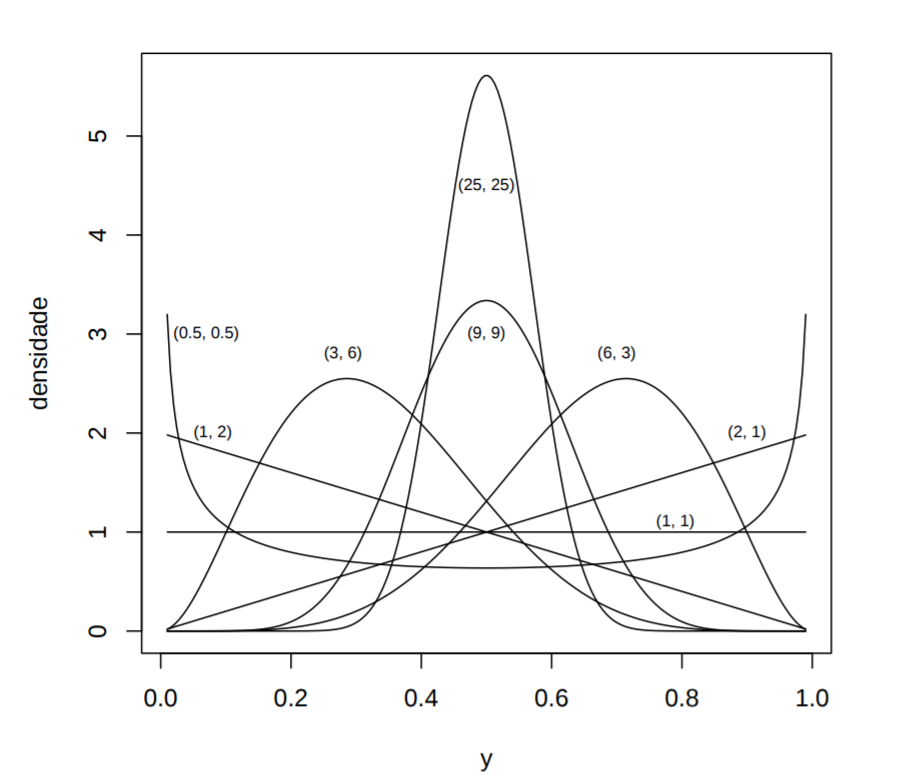
\includegraphics[keepaspectratio=true,scale=0.3]{figuras/dist-beta1.png}
	\caption{Gráfico de densidade beta para diferentes valores de $\alpha_1$ e $\alpha_2$}
	Fonte: \cite{gomes2005}
	\label{fig06}
\end{figure}


%Ao se fixar $\alpha_2$, no lado esquerdo da Fig. \ref{fig07}, é obtido a variação de densidade beta para diferentes valores de $\alpha_1$; O mesmo acontece ao se fixar o $\alpha_1$, no lado direito da Fig. \ref{fig07}, é obtido a variação de densidade beta para diferentes valores de $\alpha_2$. Ao permutar $\alpha_1$ e $\alpha_2$ ocorre uma reflexão em torno da reta $y = 0,5$, devido à expressão da densidade como função de $y$ e $y-1$. 

Se $Y$ tem distribuição beta, a média ou esperança é dada por

\begin{equation}
E(Y) = \frac {\alpha_1}{\alpha_1 + \alpha_2}
\end{equation}
%
e a variância é dada por

\begin{equation}
Var(Y) = \frac{\alpha_1\alpha_2}{(\alpha_1+\alpha_2)^2(\alpha_1+\alpha_2+1)}.
\end{equation}


%\begin{figure}[!h]
%	\centering
%	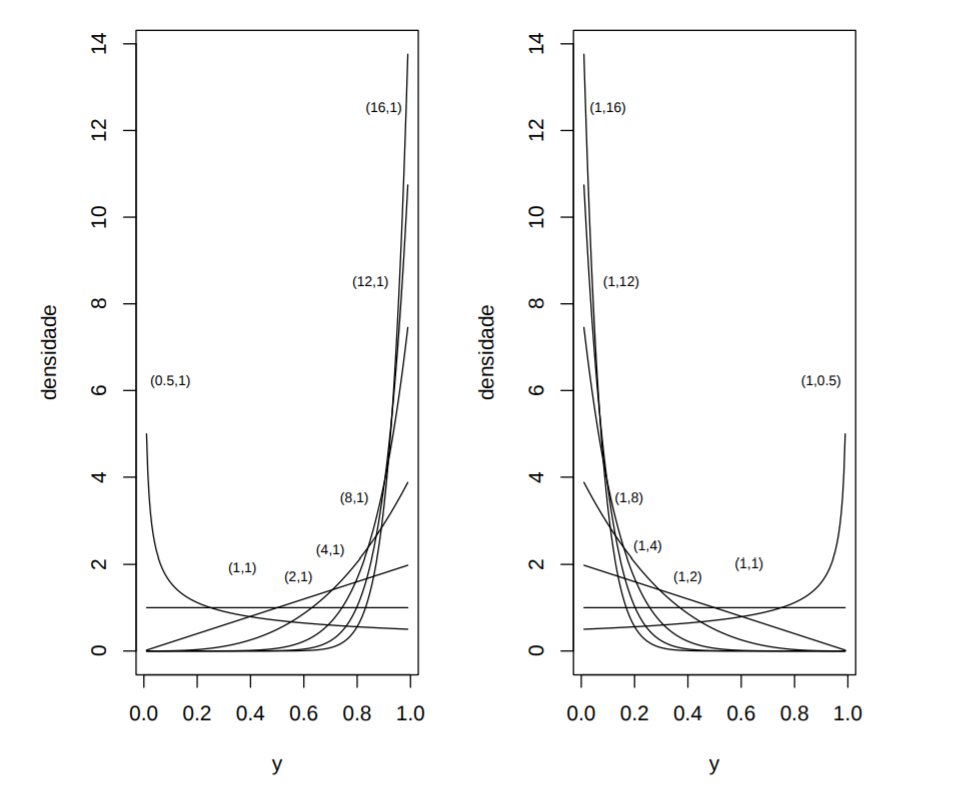
\includegraphics[keepaspectratio=true,scale=0.4]{figuras/dist-beta2.png}
%	\caption{Gráfico de densidade beta para diferentes valores de $\alpha_1$ e $\alpha_2$, fixando $\alpha_2 = 1$ (esquerda) e $\alpha_1 = 1$ (direita)}
%	Fonte: \cite{gomes2005}
%	\label{fig07}
%\end{figure}


Através da equação da variância pode-se observar que a variabilidade de $Y$ diminui à medida que se aumenta os valores dos dois parâmetros; pode ser visto na Fig. \ref{fig06} quando as distribuições são simétricas. A distribuição beta é muito utilizada para gerar frequências estatísticas aleatórias. No EJ, ela será utilizada para modelar a probabilidade de um indivíduo aceitar ou rejeitar um comentário qualquer.


\subsection{Distribuição Dirichlet}


A distribuição de Dirichlet é uma generalização da Beta para uma distribuição de probabilidade. Faz parte de uma família de distribuições de probabilidade multivariada contínuas, parametrizada por um vetor de parâmetros $\alpha$, denotada por $Dir(\alpha)$. É uma generalização multivariada da distribuição Beta, podendo ser empregada no estudo da distribuição de vetores aleatórios, cuja as variáveis aleatórias estejam compreendidas no intervalo (0,1) e a soma é igual a 1 \apud{lovelace1998}{barbosa2018}.

Seja $\textbf{p}$ um vetor aleatório cujos elementos somam 1, de modo que $p_{k}$ represente a proporção do item \textit{k} \cite{minka2000}. Sob o modelo de Dirichlet, com o vetor de parâmetros $\alpha$, a densidade de probabilidade em $\textbf{p}$ é

\begin{equation}
p(\boldsymbol {q}) \sim \mathcal{D}(\alpha_{1},\dots,\alpha_{k}) = \frac {\Gamma(\sum_{k} \alpha_{k})}{\prod_{k}\Gamma(\alpha_{k})} \prod_{k} q_{k}^{\alpha_{k}-1},
\end{equation}
%
onde $q_{k} > 0$ 

\begin{equation}
\sum_{k} q_{k} = 1.
\end{equation}    

O parâmetro $\alpha$ é um vetor com $P$ componentes $\alpha_k > 0$, e onde $\Gamma(x)$ é a função Gamma \cite{blei2003}.
Os parâmetros $\alpha$ são estritamente positivos e um fato importante é que as densidades marginais da distribuição Dirichlet são distribuições beta \cite{gomes2005}.

Seja $\phi = \sum_{i=1}^{N} \alpha_i$, deste modo, podemos escrever a média e a variância como 


\begin{equation}
E(Y_k) = \frac{\alpha_k}{\phi}, \quad k = 1, \dots, P,
\end{equation} 

\begin{equation} \label{dir:var}
Var(Y_k) = \frac{\alpha_k(\phi-\alpha_k)}{\phi^2(\phi+1)}, \quad k = 1, \dots, p-1,
\end{equation} 

\noindent
uma variável aleatória Dirichlet $P$-dimensional 
$q$ pode assumir valores no $(P-1)$-simplexo 
(um vetor-$P$ $q$ encontra-se no $(P-1)$-simplexo se 
$q_k \geq 0$,
$\sum_{i=1}^{k} q_k =1)$. 
O Dirichlet é uma distribuição conveniente no simplexo - está na família exponencial, tem estatísticas suficientes de dimensão finita e é conjugada à distribuição multinomial \cite{blei2003}.


Para a maior compreensão da distribuição de Dirichlet, o trabalho de visualização foi replicado com base em Liu (\citeyear{liu2019}). Com $P=3$ e $2$-simplexo, $P=(\alpha_1, \alpha_2, \alpha_3)$. Cada ponta do triângulo corresponde a uma coordenada diferente. 


\begin{figure}[!h]
	\centering
	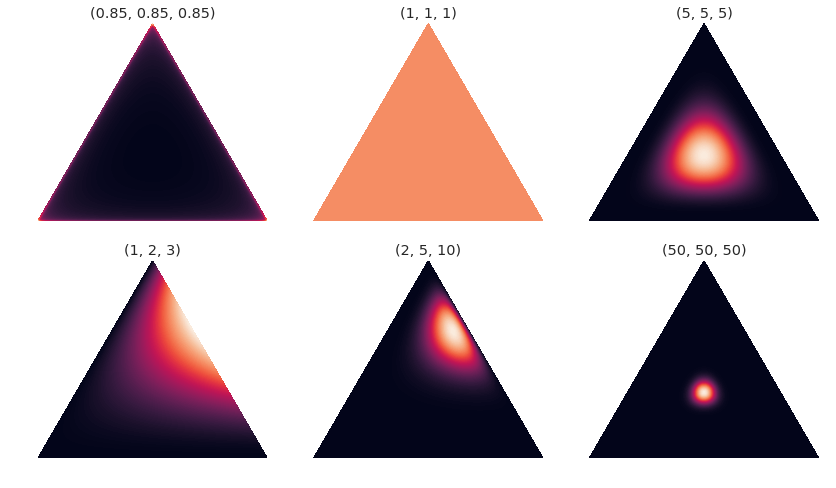
\includegraphics[keepaspectratio=true,scale=0.4]{figuras/dist-diri-simplex.png}
	\caption{Distribuição de $\alpha_1$, $\alpha_2$ e $\alpha_3$ para diferentes valores no 2-simplexo}
	\label{fig08}
\end{figure}


Em distribuições simétricas para valores de $\alpha<1$, a distruibuição se concentra nos cantos e ao longo dos limites do simplexo. No caso de $\alpha=1$, $k=(1,1,1)$, produz uma distribuição uniforme, onde todos os pontos do simplexo são igualmente prováveis. Para valores $\alpha>1$, a distribuição tende para o centro do simplexo, como pode ser visto na Fig. \ref{fig08}. Conforme $\alpha_i$ aumenta, a distribuição se torna mais concentrada em torno do centro do simplexo. 


\begin{figure}[!h]
	\centering
	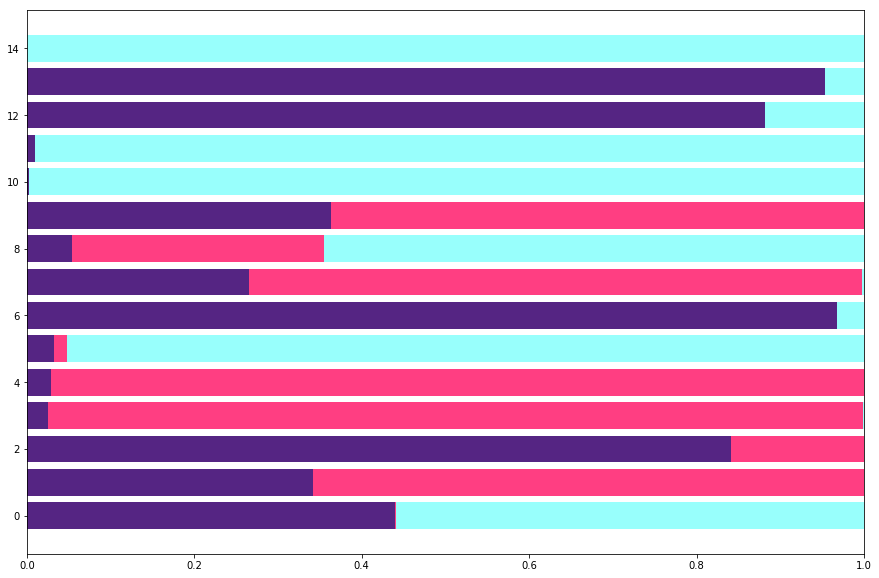
\includegraphics[keepaspectratio=true,scale=0.4]{figuras/resultados-dist-dir-01-3.png}
	\caption{Distribuição Dirichlet com $i=15$ e variações de $\alpha$ = 0,1 }
	\label{dist-dir:alpha01}
\end{figure}

Como especificado na Eq. \ref{dir:var} é possível observar que quanto maior o valor de $\alpha_i$, menor a variância. %Com três $\alpha's = 0.1$ iguais com a distribuição na Fig. \ref{dist-dir:alpha01}
Na Fig. \ref{dist-dir:alpha01} a distribuição possui três $\alpha$ iguais, onde $\alpha=0.1$ e é possível notar a maior variância na distribuição quando comparado as Fig. \ref{dist-dir:alpha1} e Fig. \ref{dist-dir:alpha10}.


\begin{figure}[!h]
	\centering
	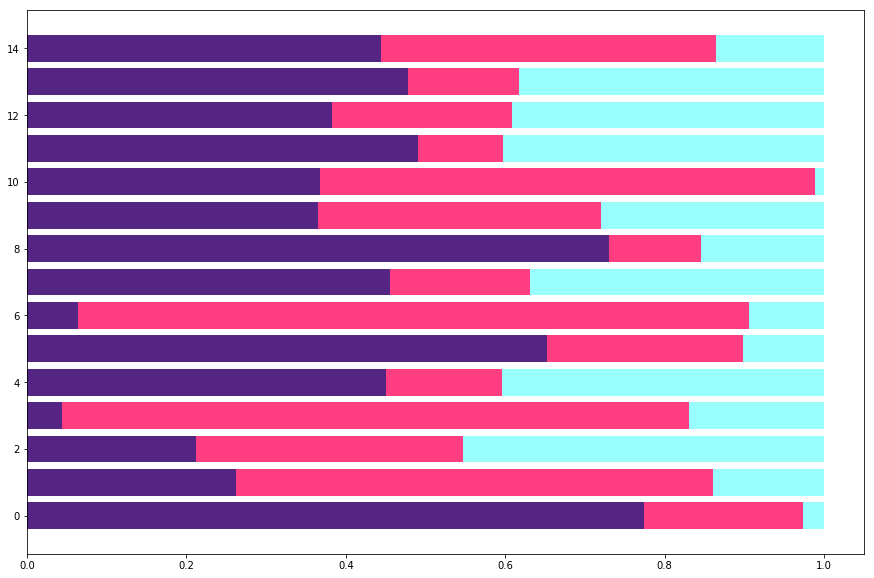
\includegraphics[keepaspectratio=true,scale=0.4]{figuras/resultados-dist-dir-1-3.png}
	\caption{Distribuição Dirichlet com $i=15$ e variações de $\alpha$ = 1 }
	\label{dist-dir:alpha1}
\end{figure}

Na Fig. \ref{dist-dir:alpha10} com $\alpha=10$ a variância diminui todos os $\alpha$ são iguais e $i=15$. Para cada distribuição, para cada $i$, $\sum_{i=1}^{3} \alpha_i = 1$.


\begin{figure}[!h]
	\centering
	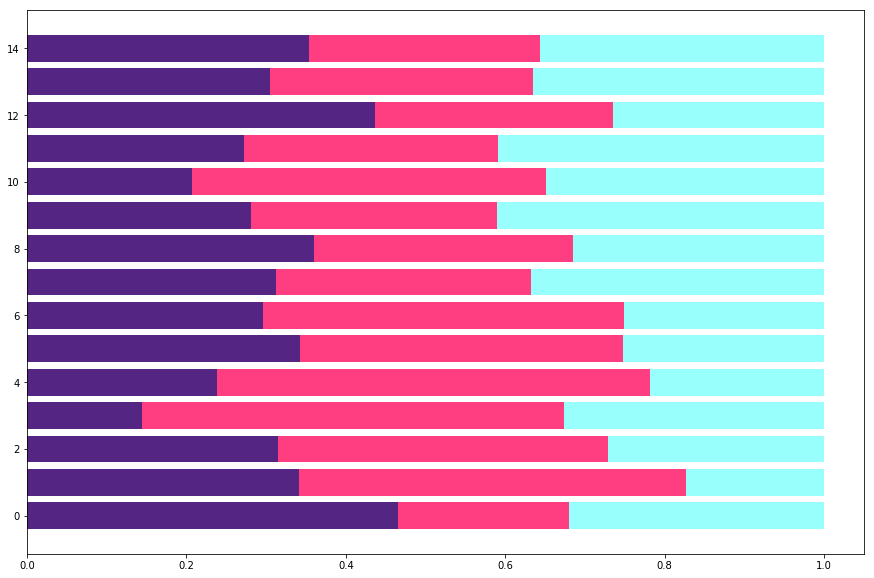
\includegraphics[keepaspectratio=true,scale=0.4]{figuras/resultados-dist-dir-10-3.png}
	\caption{Distribuição Dirichlet com $i=15$ e variações de $\alpha$ = 10 }
	\label{dist-dir:alpha10}
\end{figure}

%%% VERIFICAR CHECAR CONFIRMAR
Quanto menor o $\alpha$, maior a concentração de probabilidade em uma componente aleatória e quanto maior o $\alpha$ mais próximo todos valores ficam da média.


\section{Aprendizado de Máquina}

Aprendizado de Máquina (AM) é uma área de Inteligência Artificial (IA) cujo objetivo é o desenvolvimento de técnicas computacionais sobre o aprendizado bem como a construção de sistemas capazes de adquirir conhecimento de forma automática. Um sistema de aprendizado é um programa de computador que toma decisões baseado em experiências acumuladas através da solução bem sucedidade de problema anteriories \cite{monard2003}. 

%\cite{mitchell1997} define que um programa computacional aprende a partir da experiencia E, em relação a uma classe de tarefas T, com medida de desempenho P, se seu desempenho nas tarefas T, medida por P, melhora com a experiência E.

A indução é a forma de inferência lógica que permite obter conclusões genéricas sobre um conjunto particular de exemplos. 
Ela é caracterizada como o raciocínio que se origina em um conceito específico e o generaliza, ou seja, da parte para o todo. É um dos principais métodos utilizados para derivar conhecimento novo e predizer eventos futuros. O aprendizado indutivo é efetuado a partir de raciocínio sobre exemplos fornecidos por um processo externo ao sistema de aprendizado.

Os algoritmos de aprendizado de máquina são tipicamente classificados como supervisionados, quando são treinados a partir de um conjunto de exemplos, e não-supervisionados, quando trabalham com dados brutos sem usar um conjunto de exemplos pré-preparado.
 %O aprendizado indutivo pode ser dividido em supervisionado e não-supervisionado. 
%Os algoritmos de AM são utilizados para detecção de fraudes, análise de crédito, sistemas de recomendação, mecanismos de buscas, entre outros.
O EJ utiliza um método semi-supervisionado de classificação dos usuários em grupos de opinião. Nele, um algoritmo não supervisionado foi modificado para levar em consideração a classificação manual de um pequeno conjunto de dados.



\section{Aprendizado Supervisionada}


O aprendizado supervisionado utiliza um conjunto de exemplos de treinamento para os quais o rótulo (\textit{label}) da classe associada é conhecido.

Em geral, cada exemplo é descrito por um vetor de valores de características, ou atributos, e o rótulo da classe associada. O objetivo do algoritmo de indução é construir um classificador que possa determinar corretamente a classe de novos exemplos ainda não rotulados, ou seja, exemplos que não tenham o rótulo da classe. Para rótulos de classe discretos, esse problema é conhecido como classificação e para valores contínuos como regressão \cite{monard2003}. 


\subsection{Naive Bayes}

%O Classificador Naive Bayes é provavelmente o classificador mais utilizado em AM APUD BEM AQUI. O classificador é denominado ingênuo (\textit{naive}) por assumir que os atributos são condicionalmente independentes, ou seja, a informação de um evento não é informativa sobre nenhum outro \cite{oguri2007}. Apesar desta premissa "ingênua" e simplista, o classificador reporta o melhor desempenho em várias tarefas de classificação.

Naive Bayes é um dos mais eficientes e eficazes algoritmos de aprendizado indutivo para aprendizado de máquina e mineração de dados. É uma forma de rede Bayesiana, na qual todos os atributos são independentes, dado o valor da variável de classe. Isso é chamado de independência condicional, que raramente é verdadeira nas aplicações no mundo real. No entanto, esta aproximação muitas vezes se mostra útil e implica em um bom desempenho computacional \cite{zhang2004}.

%Uma abordagem direta para superar a limitação de ingênuos Bayes é estender sua estrutura para representar explicitamente as dependências entre os atributos.


%O bom desempenho de Naive Bayes é surpreendente, pois geralmente não reflete as aplicações do mundo real: dado o valor da classe, todos os atributos são independentes.


%O bom desempenho de Naive Bayes é surpreendente, pois faz uma suposição que quase sempre é violada em aplicações do mundo real: dado o valor da classe, todos os atributos são independentes.

Um classificador é uma função que atribui um rótulo de classe a um exemplo. Do ponto de vista da probabilidade, de acordo com a regra de Bayes, a probabilidade de um exemplo $E = (x_1, x_2, \dots, x_n)$, sendo $c$ uma classe é


\begin{equation}
p(c,E) = \frac{p(E|c)p(c)}{p(E)},
\end{equation} 
%
onde $p(c)$ é a probabilidade a priori de cada classe, $p(E|c)$ é a probabilidade do exemplo ser gerado dentro de determinada classe e $p(E)$ é uma constante de normalização.
Suponha que todos os atributos sejam independentes, dado o valor da variável de classe; isso é,

\begin{equation}
p(E|c) = p(x_1, x_2, \dots, x_n|c) = \prod_{i=1}^{n} p(x_i|c).
\end{equation}

\noindent
Naive Bayes é uma família de métodos, já que cada escolha de $p(E|c)$ e $p(c)$ produz um método diferente.

Apesar da simplicidade, Naive Bayes deve seu bom desempenho à função de perda zero-um \apud{domingos1997}{zhang2004}. Essa função define o erro como o número de classificações incorretas. Ao contrário de outras funções de perda, como o erro quadrado, a função de perda zero-um não penaliza a estimativa de probabilidade imprecisa, desde que a probabilidade máxima seja atribuída à classe correta. Isto significa que Naive Bayes pode mudar as probabilidades posteriores de cada classe, mas a classe com a probabilidade posterior máxima é muitas vezes inalterada. Assim, a classificação ainda está correta, embora a estimativa de probabilidade seja ruim \apud{friedman1997}{zhang2004}.


Zhang (\citeyear{zhang2004}) propôs uma nova explicação sobre o desempenho de classificação de Naive Bayes: a distribuição de dependência desempenha um papel crucial na classificação. Mesmo com fortes dependências, Naive Bayes ainda funciona bem; ou seja, quando essas dependências se anulam, não há influência na classificação. 

%Nesse caso, Naive Bayes ainda é o classificador ideal. 
%Além disso, investigamos a otimalidade de Naive Bayes sob a distribuição gaussiana e apresentamos a condição explícita e suficiente sob a qual Naive Bayes é ótimo, mesmo que a suposição de independência condicional seja violada.



%Neste artigo, propomos uma nova explicação sobre o desempenho de classificação de Bayes ingênuos. Mostramos que, essencialmente, a distribuição de dependência; isto é, como a dependência local de um nó distribui em cada classe, de maneira uniforme ou desigual, e como as dependências locais de todos os nós trabalham juntas, consistentemente (suportam uma certa classificação) ou inconsistentemente (anulam-se mutuamente), desempenha um papel crucial a classificação. Nós explicamos porque, mesmo com fortes dependências, Bayes ingênuo ainda funciona bem; ou seja, quando essas dependências se anulam, não há influência na classificação. Nesse caso, Bayes ingênuo ainda é o classificador ideal. Além disso, investigamos a otimalidade de Bayes ingênuos sob a distribuição gaussiana e apresentamos a condição explícita e suficiente sob a qual Bayes ingênuo é ótimo, mesmo que a suposição de independência condicional seja violada



%Os algoritmos classificadores de documentos utilizam processos indutivos. Nesta linha, um classificador para uma categoria $c_{i}$ é construído observando as características de um conjunto de documentos, previamente rotulados sob $c_{i}$ por um especialista no domínio. Esta é uma abordagem de aprendizado supervisionado, onde um novo documento é classificado de acordo com as características aprendidas por um classificador construído e treinado a partir de dados rotulados.\cite{oliveira2000} 

%Um classificador é uma função que atribui um rótulo de classe a um exemplo. Do ponto de vista da probabilidade, segundo a Regra de Bayes, a probabilidade de um exemplo $E = (x_1, x_2, \dots, x_n)$ com classe $c$ é


%O classificador AAAAAAAAAAAAAAAAAAAAAAAAAAAAAAAAAAA

%Suponha que se conheça a probabilidade prévia (\textit{a priori}) $P(w_j)$ e a densidade condicional $p(x|w_j)$

%A fórmula de Bayes:


%begin{equation}
%P(w_j,x) = \frac{p(x|w_j)P(w_j)}{p(x)}
%end{equation} 

%A fórmula de Bayes mostra que observando o valor de $x$ pode-se converter a probabilidade \textit{a priori} $P(w_j)$ para a probabilidade \textit{a posteriori} $P(w_j|x)$ - a probabilidade do estado natural de $w_j$, dado que o valor $x$ da característica tem sido medido. 

%O Classificador Naive Bayes é provavelmente o classificador mais utilizado em AM APUD BEM AQUI. O classificador é denominado ingênuo (\textit{naive}) por assumir que os atributos são condicionalmente independentes, ou seja, a informação de um evento não é informativa sobre nenhum outro \cite{oguri2007}. Apesar desta premissa "ingênua" e simplista, o classificador reporta o melhor desempenho em várias tarefas de classificação.


%https://scikit-learn.org/stable/modules/naive_bayes.html

%http://www.cs.unb.ca/~hzhang/publications/FLAIRS04ZhangH.pdf
\subsection{Processo Bernoulli}

O processo de Bernoulli pode ser visualizado como uma sequência independente de jogadas de moedas, onde a probabilidade de cara em cada jogada é um número fixo $p$ na faixa $0 < p < 1$. Em geral, o processo de Bernoulli consiste em uma sequência de tentativas de Bernoulli, onde cada tentativa produz um 1 (um sucesso) com probabilidade $p$, e um 0 (falha) com probabilidade $1 - p$, independentemente do que acontece em outros ensaios \cite{bertsekas2008}.

Naturalmente, o lançamento de moeda é apenas um paradigma para uma ampla gama de contextos envolvendo uma seqüência de resultados binários independentes. Por exemplo, um processo de Bernoulli é freqüentemente usado para modelar sistemas envolvendo chegadas de clientes ou trabalhos em centros de serviços. O tempo é discretizado em períodos, e um “sucesso” na tentativa $k$ está associado à chegada de pelo menos um cliente no centro de serviços durante o $k$-ésimo período.

Em uma descrição mais formal, é definido o processo de Bernoulli como uma sequência $X1, X2, \dots$ de variáveis aleatórias independentes de Bernoulli $X_{i}$ com

$$P(X_{i} = 1) = \textbf{P}(\textit{sucesso na i-ésima tentativa}) = p, $$
$$P(X_{i} = 0) = \textbf{P}(\textit{falha na i-ésima tentativa}) = 1-p, $$

\noindent
para cada $i$. Generalizando a partir do caso de um número finito de variáveis aleatórias, a independência de uma sequência \textit{infinita} de variáveis aleatórias de $X_i$ é definida pela exigência de que as variáveis aleatórias $X_1, X_2, \dots$ seja independentes para qualquer $n$ finito.


%\subsection{Independência e ausência de memória}
\begin{itemize}
	\item Independência e ausência de memória
\end{itemize}

O pressuposto de independência por trás do processo de Bernoulli tem implicações importantes, incluindo propriedade de ausência de memória (o que quer que tenha acontecido em testes anteriores não fornece informações sobre os resultados de ensaios futuros). Uma apreciação e compreensão intuitiva de tais propriedades é muito útil e permite a rápida solução de muitos problemas que seriam difíceis com uma abordagem mais formal.

Com duas variáveis aleatórias desse tipo e se os dois conjuntos de tentativas que os definem não tiverem um elemento comum, essas variáveis aleatórias serão independentes. Se duas variáveis aleatórias $U$ e $V$ são independentes, então quaisquer duas funções delas, $g(U)$ e $h(V)$, também são independentes \cite{bertsekas2008}.

Supondo que um processo de Bernoulli tenha sido executado por $n$ vezes, e que tenha sido observado os valores experimentais de $X_1, X_2, ..., X_n$. É notado que a sequência de futuros ensaios $X_{n + 1}, X_{n + 2}, ...$ são ensaios independentes de Bernoulli e, portanto, formam um processo de Bernoulli. Além disso, esses testes futuros são independentes dos anteriores. \cite{bertsekas2008} conclui que, a partir de qualquer dado momento, o futuro também é modelado por um processo de Bernoulli, independente do passado. Se faz referência assim, a como a propriede de novo início do processo de Bernoulli.

\subsection{Modelo Bernoulli}

O modelo multivariado de Bernoulli é uma rede Bayesiana sem dependências entre palavras e recursos de palavras binárias,
que gera um indicador para cada termo do vocabulário. Seja $1$ para indicar a presença do termo no documento ou $ 0 $ para indicar ausência.
Como o modelo multinomial, esse modelo é popular para tarefas de classificação de documentos \cite{nigam1998}.

O modelo não captura o número de vezes que cada palavra ocorre e inclui a probabilidade de não ocorrência de palavras que não aparecem no documento.

No contexto deste trabalho, o modelo de Bernoulli pode descrever bem um conjunto de interações de um usuário com duas categorias - concorda e discorda - e diversas variáveis, uma para cada comentário.


%No evento de modelo multivariado de Bernoulli, um documento é um vetor binário. Dado um vocabulário V, cada dimensão de espaço \textit{t}, $t E {1, \dots, |V|}$, corresponde a palavra $w_t$ do vocabulário. A dimensão \textit{t} do vetor de documento $d_i$ é escrita $B_{it}$, pode ser $0$ ou $1$, indicando se a palavra $w_t$ ocorre pelo menos uma vez no documento. Com essa representação de documento 


%Segundo \cite{manning2008} o modelo de Bernoulli ou  modelo multivariado de Bernoulli
%, como uma alternativa ao modelo multinomial,
%é equivalente ao modelo de independência binária, que gera um indicador para cada termo do vocabulário. Seja $1$ para indicar a presença do termo no documento ou $ 0 $ para indicar ausência. %Já o modelo multinomial captura informações de frequência de palavras em documentos. %A Figura 13.3 apresenta algoritmos de treinamento e teste para o modelo de Bernoulli. O modelo de Bernoulli tem a mesma complexidade de tempo que o modelo multinomial.


%modelo não captura o número de vezes que cada palavra ocorre e inclui explicitamente a probabilidade de não ocorrência de palavras que não aparecem no documento.


%Com essa representação de documento, a suposição de Naive Bayes: que a probabilidade de cada palavra que ocorre em um documento é independente da ocorrência de outras palavras em um documento.

%Esse modelo não captura o número de vezes que cada palavra ocorre e inclui explicitamente a probabilidade de não ocorrência de palavras que não aparecem no documento


\section{Aprendizado Não Supervisionada}

Já no aprendizado não-supervisionado, o indutor analisa os exemplos fornecidos e tenta determinar se alguns deles podem ser agrupados, formando agrupamentos ou \textit{clusters} distintos. Após a determinação dos agrupamentos, normalmente, é necessária uma análise para determinar o que cada agrupamento significa no contexto do problema que está sendo analisado \cite{monard2003}.



O número de estratégias diferentes para a formação de \textit{cluster} é enorme, e muitas abordagens podem utilizar diferentes métricas para determinar o que a "similaridade" entre os elementos nos dados significa. Algoritmos não supervisionados são capazes de descobrir a estrutura por conta própria explorando semelhanças ou diferenças (como distâncias) entre pontos de dados individuais em um conjunto de dados, são um exemplo \cite{cios2007}. Técnicas de \textit{clustering} podem ser divididos em três principais categorias: Partição, \textit{Clustering} Hierárquico e \textit{Model-based Clustering}.




\subsection{Análise de Componentes Principais}

A análise de componentes principais (PCA), do inglês Principal Component Analysis, é uma técnica multivariada de modelagem da estrutura de covariância \cite{sandanielo2015}. 
% A técnica foi inicialmente descrita por Pearson (1901) e uma descrição de métodos computacionais práticos veio muito mais tarde com Hotelling (1933, 1936) que usou com o propósito determinado de analisar as estruturas de correlação. 
O PCA transforma linearmente um conjunto
original de variáveis, inicialmente correlacionadas  entre si, num conjunto substancialmente menor de variáveis não correlacionadas que contém a maior parte da informação do conjunto original. 

É a técnica mais conhecida e
está associada à ideia de redução de massa de dados, com menor perda possível da
informação. Procura-se redistribuir a
variação observada nos eixos originais de
forma a se obter um conjunto de eixos
ortogonais não correlacionados \apud{manly1986}{sandanielo2015} \apud{hongyu2015}{sandanielo2015}.


O PCA consiste em transformar
um conjunto de variáveis originais em outro
conjunto de dimensão reduzida denominadas de componentes principais.
Os componentes principais apresentam
propriedades importantes: cada
componente principal é uma combinação linear de todas as variáveis originais, são
independentes entre si e estimados com o
propósito de reter, em ordem de estimação,
o máximo de informação, em termos da
variação total contida nos dados
\apud{wichern1998}{sandanielo2015}   \apud{hongyu2015}{sandanielo2015}.

%O objetivo principal da análise de componentes principais é o de explicar a estrutura da variância e covariância de um vetor aleatório, composto de \textit{p}-variáveis aleatórias, por meio de combinações lineares das variáveis originais. Essas combinações lineares são chamadas de componentes principais e são não correlacionadas entre si \cite{sandanielo2015}.

As técnicas de análise multivariada podem ser
utilizadas para resolver problemas como redução da dimensionalidade das variáveis, agrupar os
indivíduos (observações) pelas
similaridades, em diversas áreas do
conhecimento, por exemplo, agronomia,
fitotecnia, zootecnia, ecologia, biologia,
psicologia, medicina, engenharia florestal,
etc.

Um outro uso muito importante está na visualização. Com o PCA, podemos reduzir um conjunto de alta dimensionalidade para $2$ ou $3$ componentes e projetar estas componentes em um gráfico. O PCA preserva relações geométricas entre os pontos e muitas vezes permite a identificação visual de agrupamentos e outras formas de estruturação de dados.

\subsection{Latent Dirichlet Allocation}

A Alocação de Dirichlet Latente, do inglês Latent Dirichet Allocation (LDA), foi um modelo proposto inicialmente para ancestralidade em genética de populações, mas posteriormente foi desenvolvido de forma independente pela comunidade de processamento de textos para classificação de tópicos. 
LDA é um modelo probabilístico generativo de um corpus. A idéia básica é que os documentos são representados como misturas aleatórias sobre tópicos latentes, onde cada tópico é caracterizado por uma distribuição sobre palavras \cite{blei2003}.

No contexto do EJ, discutiremos a probabilidade de um usuário aceitar um comentário, sabendo que pertence a uma mistura de grupos de opinões.
%O LDA aplicado a este trabalho, existem as entidades comentário, usuário e grupo de opinião, que são referidas respectivamente como "palavra", "documento" e "tópico" quando vinculado ao texto. 
Considere uma conversa com $i \in [0,N]$ usuários cadastrados, $j \in [0.M]$ comentários e $k \in [0,P]$ grupos de opiniões.

A probabilidade do usuário $i$ concordar com o comentário $j$ é dada por 

\begin{equation} \label{lda:sumQF}
W_{ij} = \sum_{k} {Q}_{ik}{F}_{kj},
\end{equation}

\noindent
onde a fração da opinião $k$ do usuário é representado por ${Q}_{ik}$ e ${F}_{kj}$ representa a probabilidade de concordar com o comentário $j$. As probabilidades $Q_{ik}$ resultam em um, assim como na distribuição Dirichlet, 

\begin{equation}
\sum_{k} {Q}_{ik} = 1.
\end{equation}

%A probabilidade do usuário "ideal" do grupo $k$ concordar com o comentário $j$ é $\textbf{F}_{kj}$.

Assumimos que todos os comentários, neste primeiro momento, estão preenchidos com as opções concordar e discordar, respectivamente, $1$ e $0$. ${D}_{ij} \in [0,1]$ indica que a opção do usuário $i$ no comentário $j$. 
Com isto, podemos escrever a probabilidade.
Consideramos a matriz

%\begin{equation}
%P(\textbf{F}, \textbf{Q} | \textbf{d}) = \frac {P(\textbf{F},\textbf{Q})P(\textbf{d}|\textbf{F},\textbf{Q})} {P(\textbf{d})}
%\end{equation}

%A partir dosPara identificar a probabilidade de um comentário 

\begin{equation}
 P({D}_{ij}| {F}, {Q})= 
  \begin{cases}
     W_{ij} & \quad {D}_{ij} = 1  \\
     1-W_{ij} & \quad {D}_{ij} = 0,
  \end{cases}
\end{equation}

\noindent
onde $W_{ij}$ é dado pela Eq. \ref{lda:sumQF}.

A probabilidade de gerar o conjunto completo de $D$ é dada pelo produtório

\begin{equation}
P(\textbf{D}|\textbf{F},\textbf{Q}) = \prod_{ij} P(D_{ij}|\textbf{F}|\textbf{Q}).
\end{equation}

\noindent
Com isso usamos a regra de Bayes para inferir as probabilidades de $\textbf{F}$ e $\textbf{Q}$:

\begin{equation}
P(\textbf{F}|\textbf{Q}) = \frac{P(\textbf{Q}|\textbf{F})P(\textbf{F})}{P(\textbf{Q})},
\end{equation}

\begin{equation}
P(\textbf{F}|\textbf{Q}) = {P(\textbf{F})P(\textbf{Q})}.
\end{equation}

A referência à distribuição de Dirichlet se dá justamente pela escolha da probabilidade a priori para $\textbf{F}$ e $\textbf{Q}$. O modelo assume que cada $F_{kj}$ é governado por uma distribuição Beta e cada vetor $Q_{i} = (Q_{i1}, Q_{i2}, \dots, Q_{iP})$ é dado por uma distribuição de Dirichlet.

%http://conteudo.icmc.usp.br/CMS/Arquivos/arquivos_enviados/BIBLIOTECA_158_RT_409.pdf

%http://www.jmlr.org/papers/volume3/blei03a/blei03a.pdf


\subsection{\textit{K-means}}


A partir de um conjunto de dados não classificados o k-means, técnica não supervisionada, tem o objetivo de encontrar dados semelhantes que estejam agrupados no mesmo \textit{cluster}. Possui o parâmetro $k$ que no algoritmo k-means representa a quantidade de agrupamentos ou \textit{clusters}. 

A utilização do k-means possui vantagem por ser rápida e facilmente implementada em larga escala. A idéia por trás do algoritmo é bastante simples. O conjunto de dados é dividido em $k$ \textit{clusters} e seus centros são calculados como a média das amostras daquele agrupamento. O centro representa cada \textit{cluster} por estar próximo de todas as amostras e, portanto, é semelhante a todas elas \cite{mucherino2009}.

No k-means o parâmetro $k$ define os pontos iniciais dos centros dos agrupamentos. É repetido o processo de formação de $k$ \textit{clusters}, cada ponto em um centróide mais próximo, e recalculado o centróide de cada cluster até que não haja mudanças. 

%Colocar algoritmo codigo portugol? Imagem? 

Existem algumas desvantagens na utilização do k-means, sendo uma dessas a determinação do parâmetro $k$. O $k$ geralmente é desconhecido, e o ideal seria o teste com variados valores de $k$ e escolher um que mostre o melhor resultado \cite{tan2005}.

%Para o projeto do EJ é preciso testar com quais Ks?

Uma métrica proposta para técnicas de particionamento é Coeficiente de \textit{Silhouette} 
que é calculado usando a distância intra-\textit{cluster} $(a)$ e a distância do \textit{cluster} mais próximo $(b)$ para cada amostra. O Coeficiente de \textit{Silhouette} para uma amostra é $(b-a)/max(a,b)$ 
%, com o número de agrupamentos 
e é definido apenas se o número de agrupamentos for maior que $2$ e menor que o tamanho da amostra $- 1$.

O melhor valor para o coeficiente é $1$ e o pior valor é $-1$. Valores próximos a $0$ indicam clusters sobrepostos. Valores negativos geralmente indicam que uma amostra foi atribuída ao cluster errado, pois um cluster diferente é mais semelhante 
\footnote{\href{https://scikit-learn.org/stable/modules/generated/sklearn.metrics.silhouette_score.html}{https://scikit-learn.org/stable/modules/generated/sklearn.metrics.silhouette\underline{\space}score.html}}.
%Essa silhueta mostra quais objetos ele está bem dentro do cluster e quais estão apenas em algum lugar entre os clusters.
Este valor também fornece uma avaliação da validade do \textit{cluster} e pode ser usada para selecionar um número "apropriado" de clusters \cite{rousseeuw1987}.


%A utilização do coeficiente 
%Uma nova exibição gráfica é proposta para técnicas de particionamento. Cada cluster é representado por uma chamada silhueta, que se baseia na comparação de sua estanqueidade e separação. Essa silhueta mostra quais objetos ele está bem dentro do cluster e quais estão apenas em algum lugar entre os clusters. Todo o cluster é exibido combinando as silhuetas em um único gráfico, permitindo uma apreciação da qualidade relativa dos clusters e uma visão geral da configuração dos dados. A largura média da silhueta fornece uma avaliação da validade do cluster e pode ser usada para selecionar um número "apropriado" de clusters.





\chapter{Metodologia}
\label{chap:4}


Este capítulo aborda tecnologias utilizadas para o alcance dos objetivos e a obtenção dos resultados. O estudo técnico de algoritmos e das distribuições foi colocado em prática utilizando a linguagem de programação Python, que é muito utilizada em ciência de dados.


\section{Criação de dados sintéticos}

Os dados sintéticos foram dados criados para simular um cenário real para a análise do comportamento em diferentes modelos de classificação.

Foram criados dados de usuários para diferentes grupos e votos de cada um para os comentários. As análises foram feitas em um cenário ideal, onde todos os usuários votassem que concorda ou discorda. Com observações no mundo real e no próprio EJ, o voto de concorda teve um peso maior, pois entende-se que os usuários esperam a aceitação de seus comentários.

%O voto de concorda teve um peso maior com observações no mundo real e no próprio EJ, pois os criadores de comentários esperam a aceitação

%Ainda 

%Foi criado com base em distribuições d

 %foram criados com base em 

%com base em um cenário rea

\section{Análise dos dados da plataforma}

Os dados utilizados neste trabalho foram extraídos da plataforma EJ, aplicado ao público do ENAP (Escola Nacional de Administração Pública)\footnote{\href{enap.gov.br}{enap.gov.br}} em duas conversas entre o ano de 2018 e 2019. As conversas são "Como os serviços públicos podem se adequar às demandas do cidadão do futuro?"e "O que pode ser feito para superar os desafios da transformação digital do governo?". A primeira conversa conta com 111 comentários e a segunda com 97 comentários.

No processo de entendimento e tratamento dos dados algumas dificuldades foram encontradas e solucionadas da seguinte  forma:

\begin{enumerate}
\item \textbf{Os usuários tinham apenas dados de nome e sobrenome e tinham alguns nomes vazios}: foi criado uma coluna com o gênero e preenchido manualmente com a identificação de gêneros masculino e feminino, para os usuários sem nome e com nomes que impossibilitasse a identificação de gênero foram classificados como uma terceira categoria: não identificado.
\item \textbf{Possuem identificadores de usuários iguais nas duas conversas, mas são de pessoas diferentes}: As duas conversas foram analisadas separadamente, já que não tinha como saber se um mesmo usuário respondeu ambas as conversas.
\item \textbf{Muitos comentários não foram visualizados}: Os votos possuem três reações possíveis: concordar, discordar e passar. Mas por conta do grande número de comentários não visualizados uma categoria foi criada para esses votos.
\end{enumerate}

Após a estruturação dos dados e criação de outras \textit{features} foi possível analisar a classificação de perfis dos usuários.
%Desta forma foi possível aplicar modelos não supervisionado
 

\section{Ferramentas}

A concepção deste trabalho consiste no uso de ferramentas que auxiliaram em todo o códido, resultados e análises. A ciência de dados vem conquistando entusiastas e um espaço cada vez maior no mercado juntamente com o uso da linguagem de programação Python. 

A extensa comunidade de mantenedores das bibliotecas de Python e software livre auxiliaram na escolha das ferramentas deste trabalho.
% como a popularização da liguagem de programação Python
% e as comunidades 

% utilizou Jupyter Notebook, um aplicativo Web que permite criar códigos, equações, visualizações e texto no mesmo arquivo \footnote{https://jupyter.org/}. Todo o versionamento de código foi está no repositório \footnote{https://github.com/naiieandrade/tcc-studies} do Github.

\subsection{Python}

A linguagem de programação Python \footnote{\href{https://www.python.org/}{https://www.python.org/}} foi escolhida devido ao conjunto de bibliotecas e ferramentas especializadas de aprendizado de máquina e \textit{deep learning}, que permitem aos cientistas de dados a construção de modelos sofisticados \footnote{\href{https://analyticsindiamag.com/heres-why-python-continues-to-be-the-language-of-choice-for-data-scientists/}{https://analyticsindiamag.com/heres-why-python-continues-to-be-the-language-of-choice-for-data-scientists/}}.

Inicialmente, foi analisado a distribuição Dirichlet e para isso foram utilizados as bibliotecas em Python \textbf{numpy} \footnote{\href{https://docs.scipy.org/doc/numpy/reference/generated/numpy.random.dirichlet.html}{https://docs.scipy.org/doc/numpy/reference/generated/numpy.random.dirichlet.html}} para a criação de amostras da distribuição Dirichlet, e \textbf{matplotlib} \footnote{\href{https://matplotlib.org/}{https://matplotlib.org/}} para a visualização dos dados. Matlplotlib é uma biblioteca de plotagem 2D do Python que possibilita a criação das mais diversas visualizações, várias delas são utilizadas para o melhor compreendimento dos dados. A biblioteca \textbf{scikit learn} \footnote{\href{https://scikit-learn.org/stable/modules/generated/sklearn.decomposition.PCA.html}{https://scikit-learn.org/stable/modules/generated/sklearn.decomposition.PCA.html}} foi utilizada para a construção de modelos de clusterização e de redução de dimensionalidade para o trabalho atual.

É importante ressaltar que podem existir incompatibilidade de funções em versões diferentes de bibliotecas ou ferramentas. Portanto na Tab. \ref{tab:ferramentas} está descrito as ferramentas utilizadas e suas respectivas versões para a realização deste trabalho. 

\begin{table}[!h]
\centering
\label{tab:ferramentas} 
\begin{tabular}{|c|c|}
\hline
\rowcolor[HTML]{EFEFEF} 
{\color[HTML]{333333} Ferramenta} & {\color[HTML]{333333} Versão}  \\ \hline
Python                  & 3.5.2            \\ \hline
Jupyter                  & 1.0.0 \\ \hline
Pandas                  & 0.24.2 \\ \hline
Numpy                  & 1.16.3 \\ \hline
Matplotlib                  & 3.0.3 \\ \hline
Scikit-learn                  & 0.20.3 \\ \hline
\end{tabular}
\caption{Versão de ferramentas utilizadas}
\end{table}

%As versões de todas as bibliotes utilizadas se encontram no arquivo \textbf{requirements.txt} no repositório \href{https://github.com/naiieandrade/tcc-studies}{https://github.com/naiieandrade/tcc-studies}.

\subsection{Git e Github}

O versionamento do código foi utilizado utilizando a ferramenta Git \footnote{\href{https://git-scm.com/}{https://git-scm.com/}} que possibilita rastrear o processo de desenvolvimento do código fonte e ter acesso às versões anteriores por meio do histórico de versionamento.

Além disso, foi utilizado também o Github \footnote{\href{https://github.com/}{https://github.com/}} que  é um serviço de hospedagem e repositórios Git na nuvem. Permite a criação de repositórios públicos, que possibilita a contribuição de outros interessados e mantém a transparência dos resultados.

%Um grande problema ao trabalhar com dados é a perca de informações no processo e a falta de histórico eficiente e por isso foi utilizado a ferramenta de versionamento de código Git	  e o Github .

%Todo o trabalho pode ser encontrado no repositório
%\footnote{https://github.com/naiieandrade/tcc-studies}
%Todas as mudanças estão disponíveis no histórico 


%O Git permite que a maioria de suas operações  necessitem apenas arquivos e recursos locais, e o Github é uma interface online que mantém o trabalho na nuvem, em 

%onde todo o histórico de mudanças salvas passa a estar também no servidor deles, na nuvem.

%Com o trabalho no Github é possível rastrear o processo de desenvolvimento de todo o trabalho,  criar documentos que não sejam código, manter transparência do projeto o que possibilita também a contribuição de outros usuários. 
%O histórico é mantido a cada nova mudança sendo possível também o acesso a essas versões anteriores. 




%https://github.com/ejplatform


% auxilia no fluxo de trabalho

 

\subsection{Jupyter}
%utilizou Jupyter Notebook, um aplicativo Web que permite criar códigos, equações, visualizações e texto no mesmo arquivo . Todo o versionamento de código foi está no repositório \footnote{https://github.com/naiieandrade/tcc-studies} do Github.

O Jupyter Notebook \footnote{\href{https://jupyter.org/}{https://jupyter.org/}} foi a ferramenta escolhida para trabalhar com os dados porque é um aplicativo web de código aberto que permite a criação e compartilhamento de documentos que contêm código, visualizações, equações e texto narrativo. Essas funcionalidades permitem a explicação de código e a visualização dos resultados.

%Todas essas funcionalidades foram utilizadas, 


%\section{Análise exploratória}



\chapter{Resultados}
\label{chap:5}

\section{Dados sintéticos}

A fim de entender a distribuição em um cenário próximo do real, foi simulado a existência de 4 grupos de opiniões, com 100 comentários respondidos e com $\alpha = 1$. Um vetor de $\alpha$ foi utilizado como parâmetro, $k=(2\alpha, \alpha)$, significando respectivamente comentários que concordam e discordam como mostrado na Fig. \ref{dist-dir:2alphas}. Os $\alpha$ foram escolhidos por uma hipótese de que os usuários fazem comentários desejando que estes sejam aprovados, curtidos por uma maioria. As bolhas de opinião trazem essa sensação ao usuário, de pessoas próximas e que concordem sejam a maioria para aquela realidade.



\begin{figure}[!h]
	\centering
	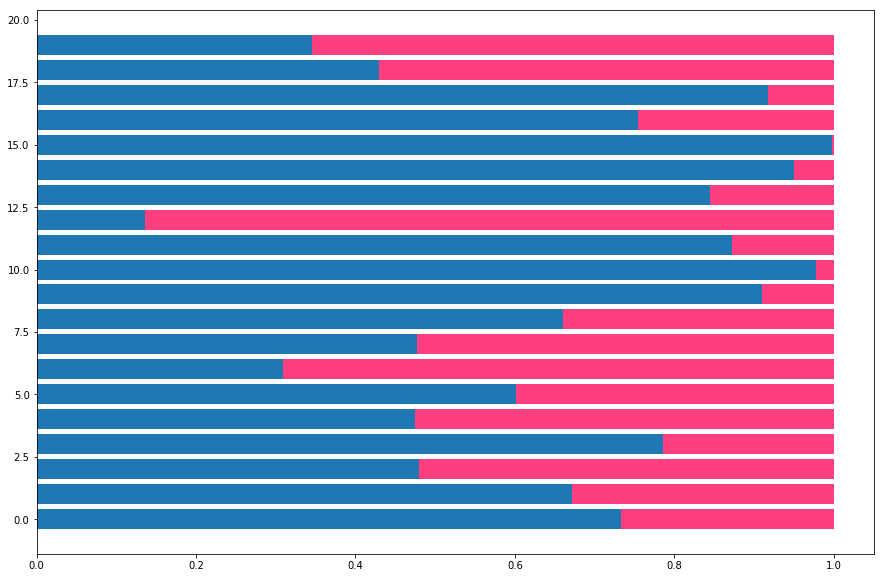
\includegraphics[keepaspectratio=true,scale=0.35]{figuras/resultados-dist-dir-2-alfas.png}
	\caption{Distribuição Dirichlet com $k=(2, 1)$}
	\label{dist-dir:2alphas}
\end{figure}



Cada grupo de opinião conta com 100 participantes, 
% totalizando 400 participantes 
que responderam os 100 comentários. Este seria um cenário ideal. E para visualizar utilizou o PCA para redução de dimensionalidade. Cada grupo de opinião foi colorido de cor distinta.

%Na Fig. \ref{pca:4-categorias} após o PCA notou se a aproximação dos usuários de cada grupo de opinião e aproximidade entre

\begin{figure}[!h]
	\centering
	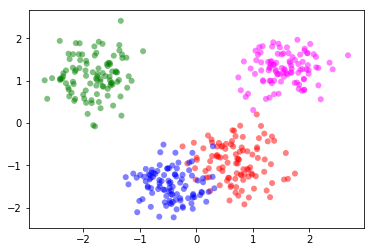
\includegraphics[keepaspectratio=true,scale=0.65]{figuras/resultados-pca-1.png}
	\caption{Grupos de opinião sintéticos utilizando redução de dimensionalidade}
	\label{pca:4-categorias}
\end{figure}



\section{Testes dos modelos de classificação}

Foi realizado uma análise da utilização do Naive Bayes com um modelo de Bernoulli  %\footnote{https://scikit-learn.org/stable/modules/generated/sklearn.naive_bayes.BernoulliNB.html}, problema no NAIVE_BAYES
considerando que os votos de cada comentário são independentes. Na Fig. \ref{pca:acc-bernoulli} é possível visualizar o aumento da acurácio do modelo. Este modelo possui  treino de teste, que foi especificado como $1/5$ dos votos.


\begin{figure}[!h]
	\centering
	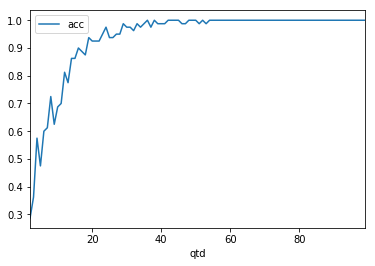
\includegraphics[keepaspectratio=true,scale=0.6]{figuras/resultados-pca-acc.png}
	\caption{Acurácia definida como o número de classificações certas / total de classificações}
	\label{pca:acc-bernoulli}
\end{figure}


Com o estudo e análise de variações do $\alpha$, quanto ao gráfico da acurária, que com um $\alpha$ maior, maior é a variação e a necessidade de mais dados para que venha a convergir a 1. 

Foi comparado também a variação de $\alpha$ para a análise do gráfico de acurácia quanto aos comentários. Nestes casos, a fim de simular os dados reais, não existem dados de treino. A acurácia é definida como o número de classificações certas / total de classificações.

\begin{figure}[!h]
	\centering
	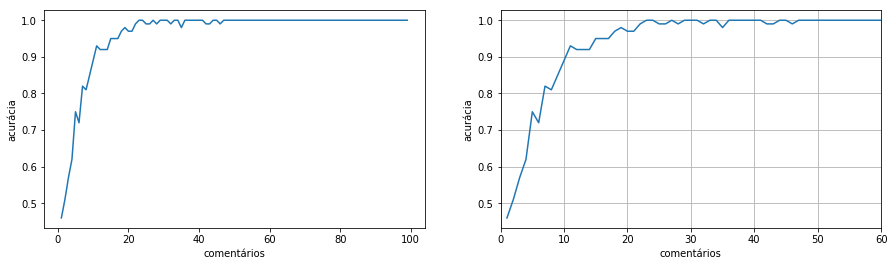
\includegraphics[keepaspectratio=true,scale=0.480]{figuras/compare-diri-1.png}
	\caption{Acurácia com os parâmetros de $\alpha = (1, 1)$}
	\label{compare:diri-1}
\end{figure}

\begin{figure}[!h]
	\centering
	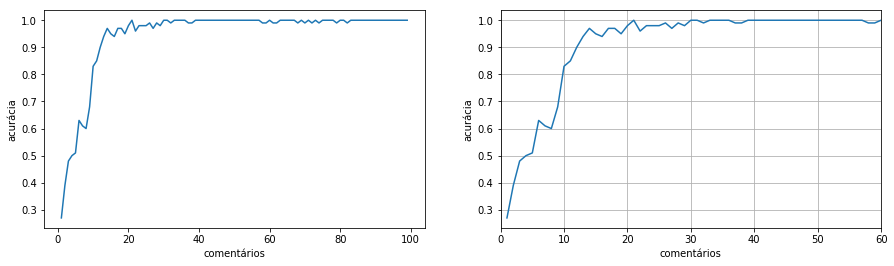
\includegraphics[keepaspectratio=true,scale=0.480]{figuras/compare-diri-2.png}
	\caption{Acurácia com os parâmetros de $\alpha = (2, 1)$}
	\label{compare:diri-2}
\end{figure}

Na Fig. \ref{compare:diri-10} quanto maior o $\alpha$, maior as oscilações de acurácia e o atraso da convergência $\alpha = 1$ quando comparado as Fig. \ref{compare:diri-1} e Fig. \ref{compare:diri-2}.

\begin{figure}[!h]
	\centering
	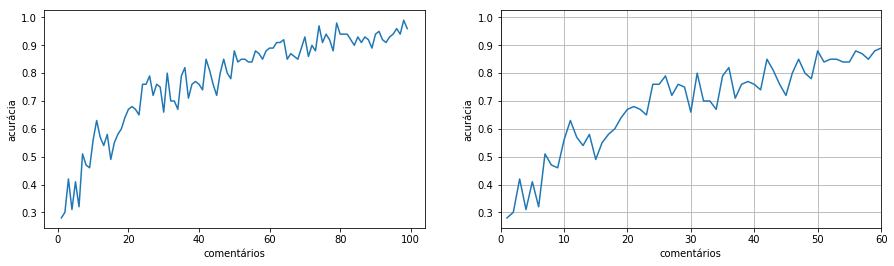
\includegraphics[keepaspectratio=true,scale=0.480]{figuras/compare-diri-3.png}
	\caption{Acurácia com os parâmetros de $\alpha = (10, 1)$}
	\label{compare:diri-10}
\end{figure}


%\newpage
\section{Dados reais}
\label{chap:dados-reais}

Para este trabalho foram cedidos dados para análises de duas conversas aplicados em um contexto atual e real da plataforma EJ. Cada conversa contém comentários criados pelos próprios usuários a fim de propor uma solução. Os comentários são utilizados para expressar concordância, discordância ou nenhum dos dois, que seria a opção de passar o comentário.

%A análise que se segue será feita em cima de duas conversas realizadas com o público da ENAP. As conversas são "Como os serviços públicos podem se adequar às demandas do cidadão do futuro?" e "O que pode ser feito para superar os desafios da transformação digital do governo?".


\begin{table}[!h]
\centering
\begin{tabular}{|c|c|c|}
\hline
                           & \textbf{Conversa 01} & \textbf{Conversa 02} \\ \hline
Votos totais               & 5480                 & 3189                 \\ \hline
Comentários únicos         & 111                  & 97                   \\ \hline
Usuários únicos            & 395                  & 184                  \\ \hline
Porcentagem de concordar    & 61,09 \%                   & 54,87 \%                   \\ \hline
Porcentagem de pular &    31,82 \%              & 39,54 \%                   \\ \hline
Densidade de votos            & 0,1249                  & 0,1786                  \\ \hline
Média de votos por usuário            & 13,87                  & 17,33                  \\ \hline
Média de votos por comentário            & 49,36 & 32,87                  \\ \hline

\end{tabular}
\caption{Dados comparativos das duas conversas analisadas}
\label{tab:dados-comparativos-conversas}
\end{table}

 
Na Tab. \ref{tab:dados-comparativos-conversas} podemos encontrar alguns dados comparativos, como votos totais por conversa, quantidade de comentários, entre outros. 
Os dados validam a hipótese de que os usuários tem maior propensão a concordarem com os comentários, aproximadamente $61\%$ e $55\%$ respectivamente. A opção de pular também é mais executada do que a de discordar.
A densidade dos votos é a razão da quantidade total dos votos por a quantidade máxima de votos por conversa, ou seja o caso ideal de todos os usuários votarem todos os comentários. A densidade traz um valor considerado baixo em uma escala $[0,1]$.




Os dados dos usuários foram separados por conversas, entretanto, existem identificadores iguais para usuários diferentes, o que invalida a possibilidade de analisar todos os usuários em conjunto, assim como saber se um mesmo usuário respondeu às duas conversas. Então as análises foram realizadas para cada conversa.

A Fig. \ref{fig:hist-compara-votos-conversas} é um histograma com a distribuição de frequências, que traz da quantidade de votos totais pela frequência de usuários únicos.  
%demostra a quantidade de votos por usuários.
A concentração inicial dos votos abrange cerca de $40\%$ dos usuários, dos quais responderam até 5 comentários. %Cerca de 40\% dos usuários, de ambas as conversas, responderam até 5 comentários.


\begin{figure}[!h]
	\centering
	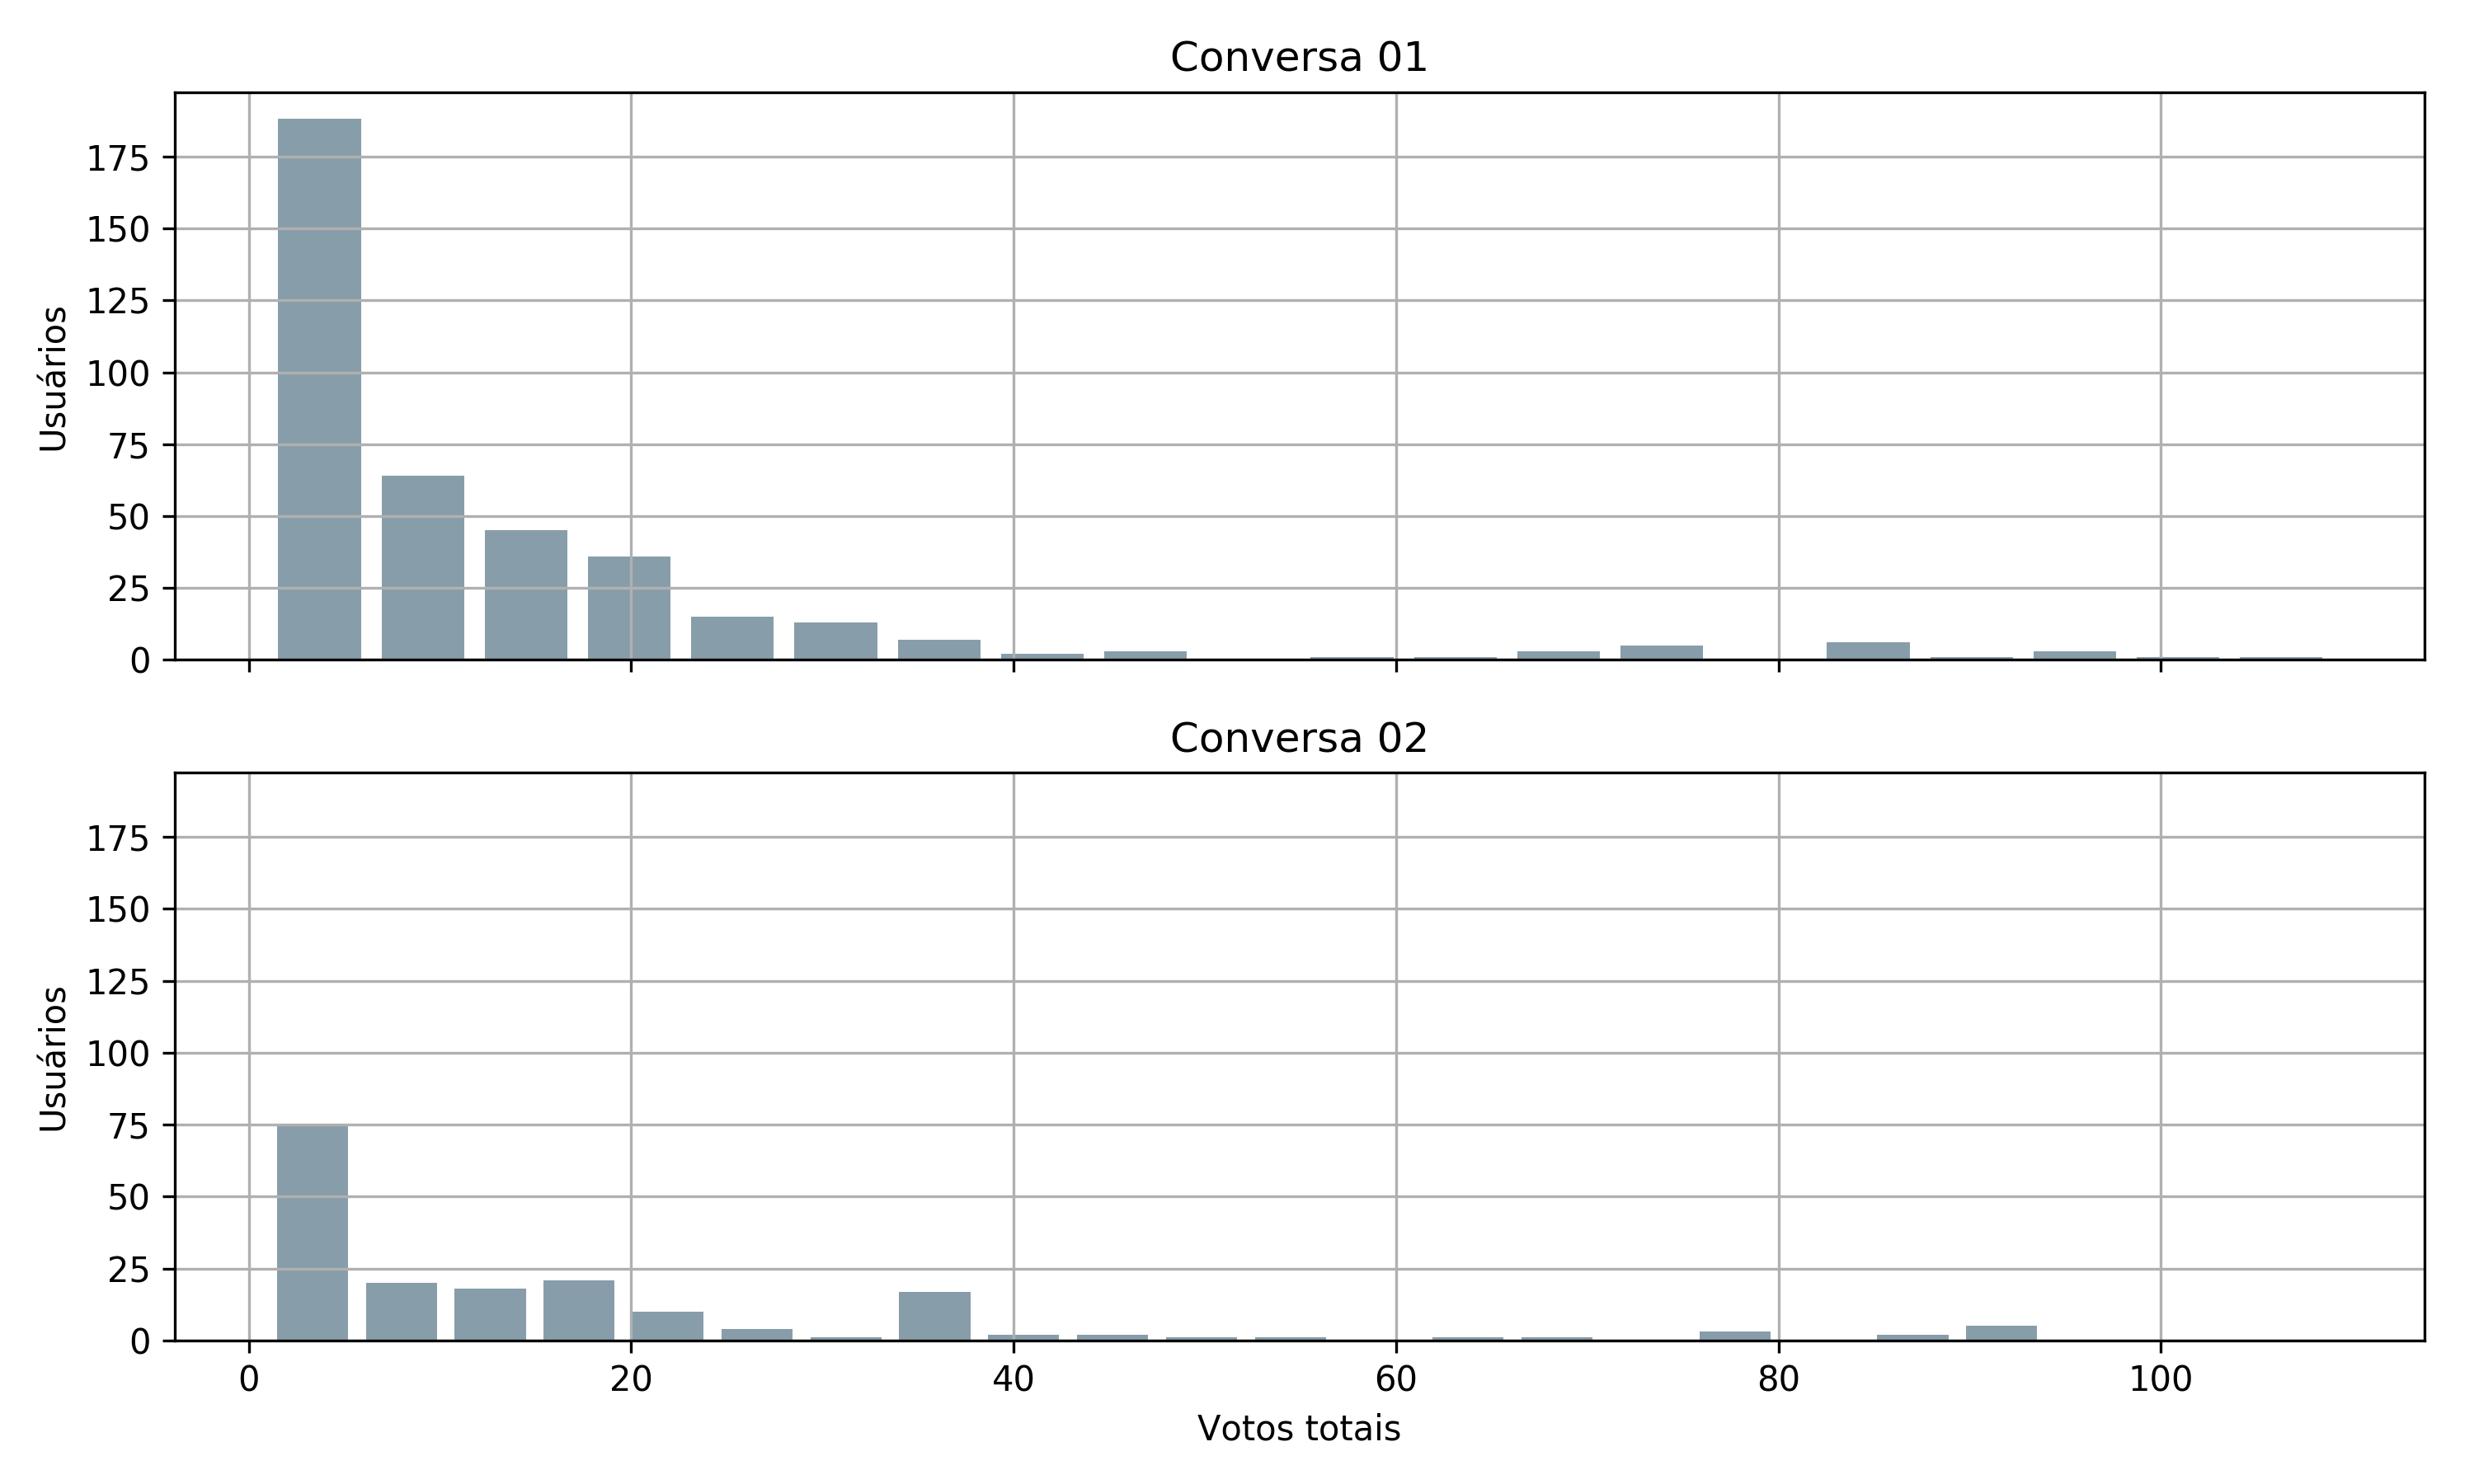
\includegraphics[keepaspectratio=true,scale=0.60]{figuras/tcc2/histogram_comparative_votes_per_user.png}
	\caption{Quantidade de votos por usuários}
	\label{fig:hist-compara-votos-conversas}
\end{figure}


\begin{figure}[!h]
	\centering
	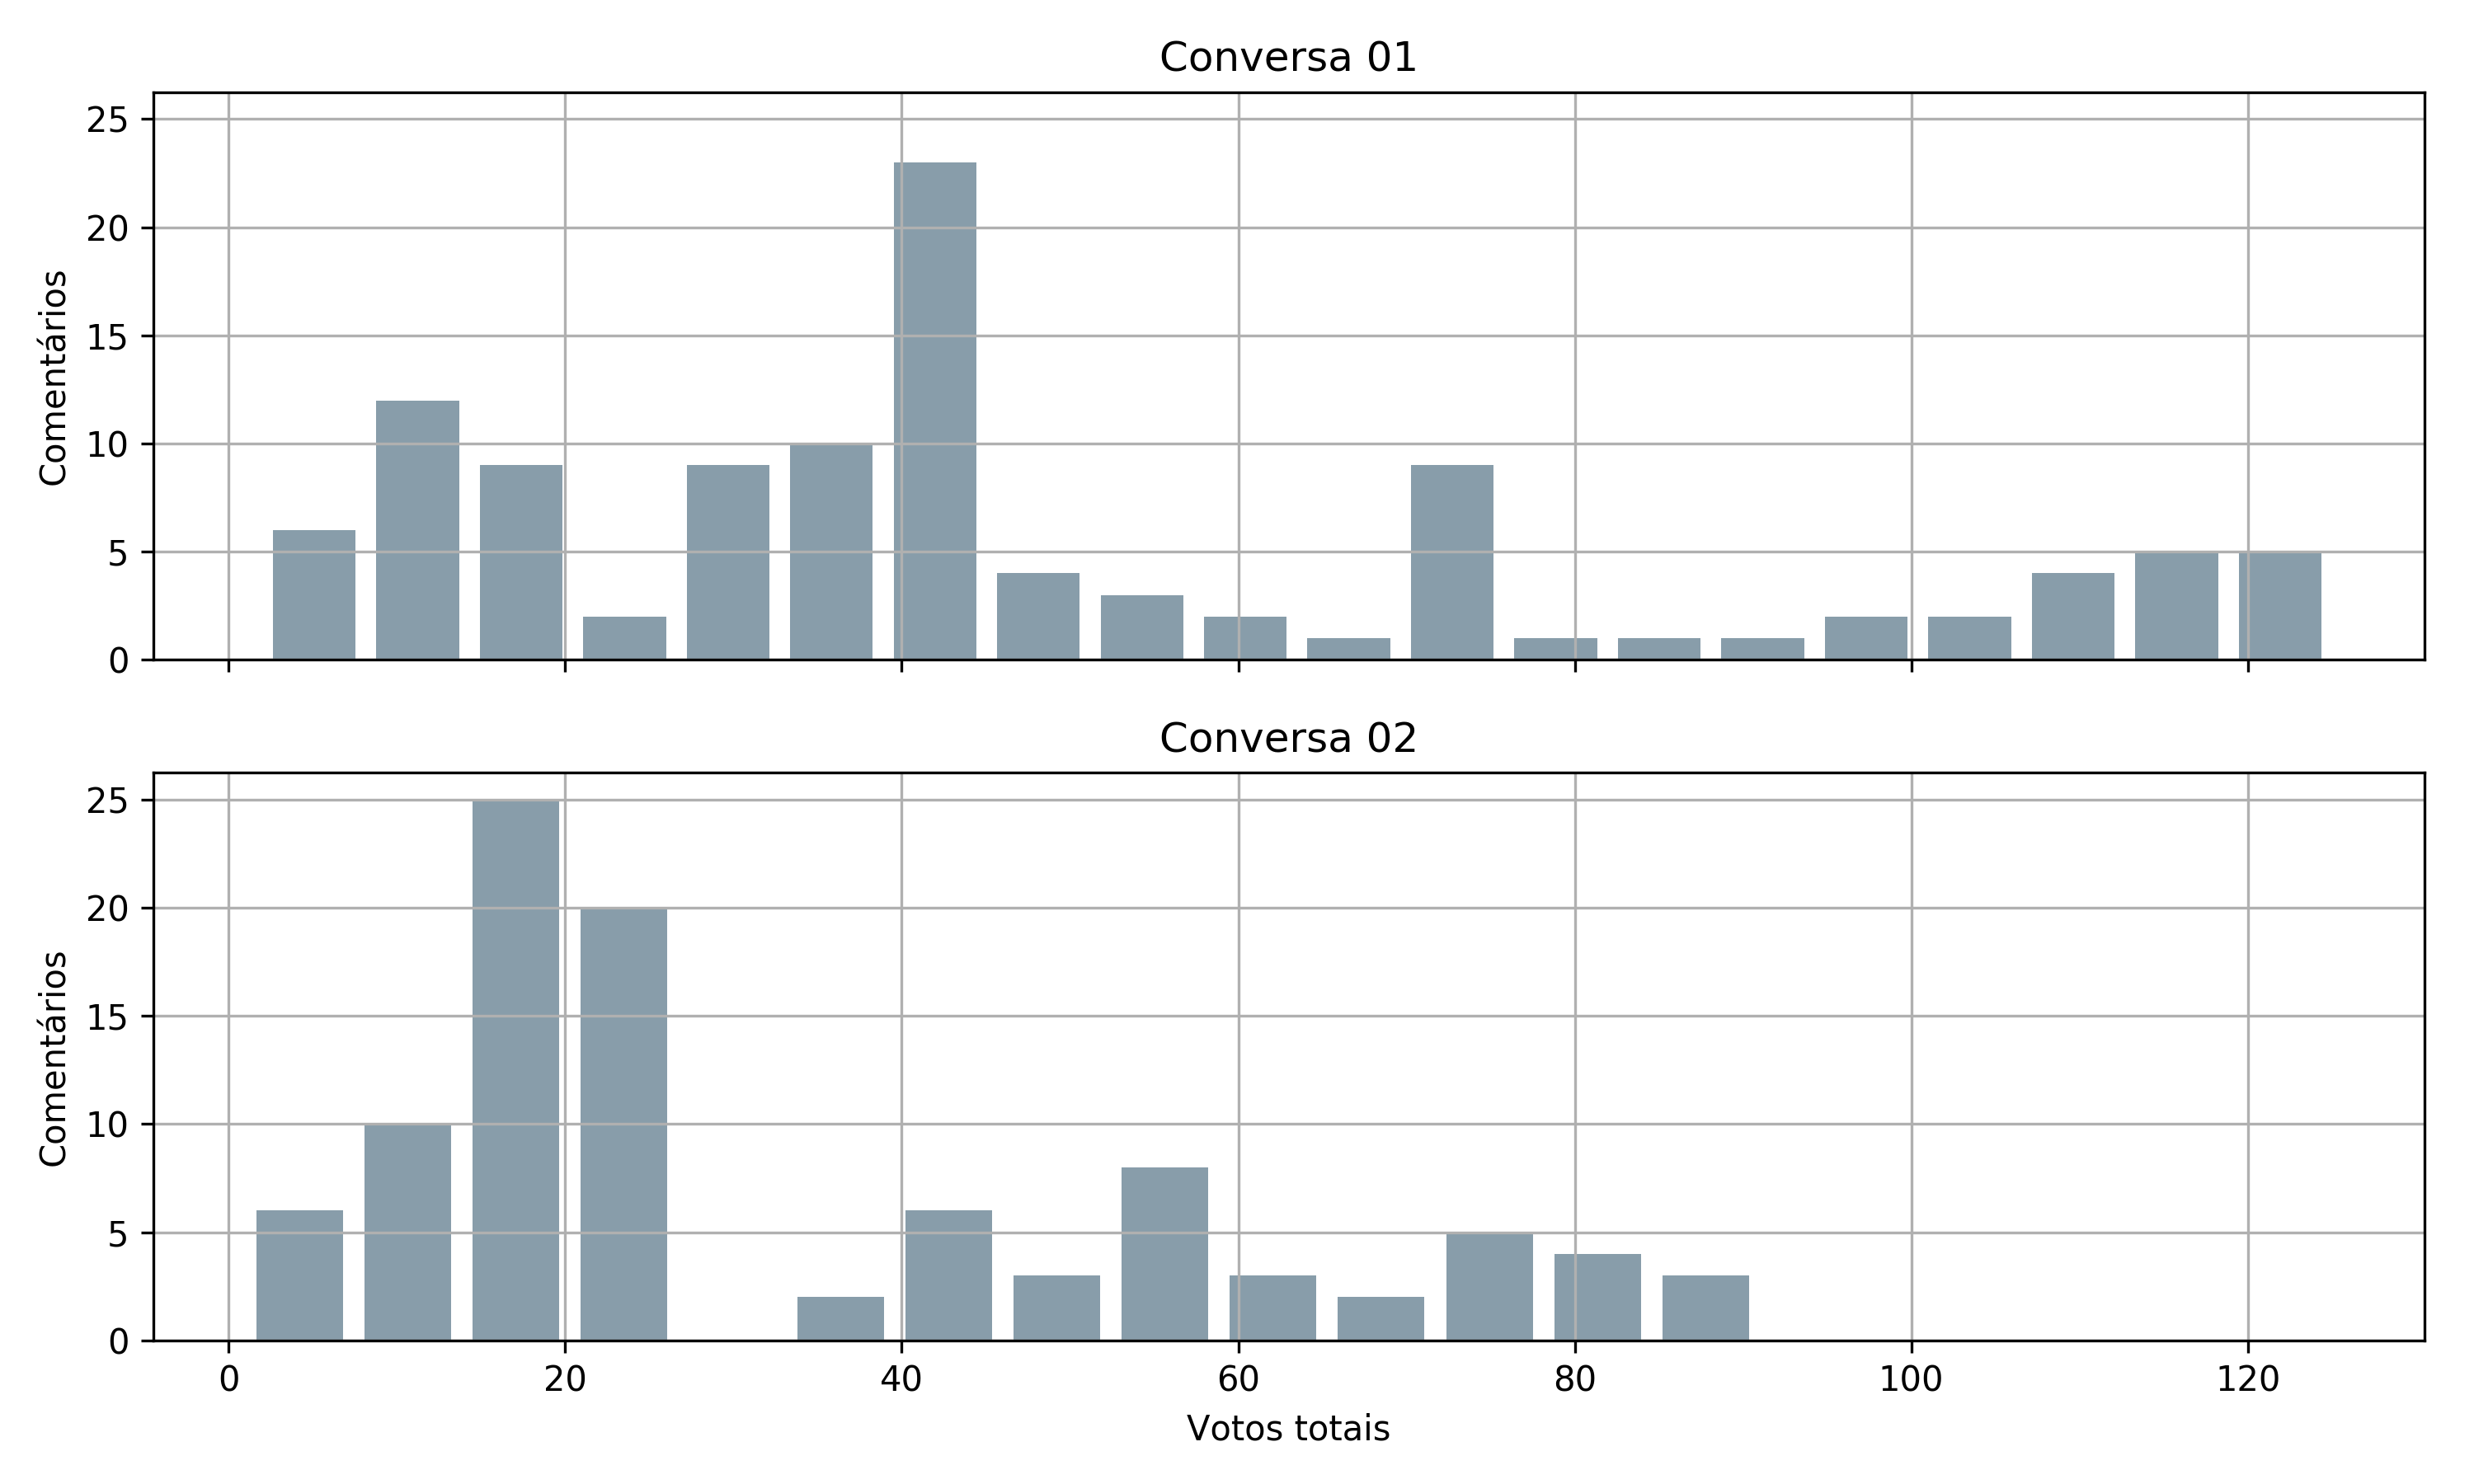
\includegraphics[keepaspectratio=true,scale=0.60]{figuras/tcc2/histogram_comparative_votes_per_comment.png}
	\caption{Quantidade de votos por comentários}
	\label{fig:hist-compara-votos-comentarios}
\end{figure}


Na Fig. \ref{fig:hist-compara-votos-comentarios} o histograma traz quantidade de votos totais pela frequência de comentários únicos. Na Conversa 01 e Conversa 02, os comentários que tiveram até $20$ votos totais até representam respectivamente $24\%$ e $42\%$ de todos os comentários de cada conversa.


Na plataforma, uma conversa promove um tema e dentro de cada conversa pode-se criar quantos comentários cada usuário quiser. Esses comentários atualmente passam por uma curadoria, que é realizada pela própria equipe de desenvolvimento, a fim de que não haja comentários iguais ou que viole o termo de uso. 
Para votar os usuários não precisam necessariamente terem criado algum comentário. 

Os votos são representados numericamente por $-1$, $0$, e $1$, associados respectivamente as opções de discordar, passar e concordar. Entretanto, os dados revelam que existem muitos comentários não respondidos, ou seja, se quer foram visualizados. Como por exemplo, na Conversa 01 o comentário mais votado possui a participação aproximadamente de $30\%$ dos usuários, já a Conversa 02 conta com 
% uma participação máxima
quase a metade dos participantes da conversa. A partir dessas informações pode-se identificar a parcela significante de comentários não vistos.
%e na Conversa 02 
%Já a Conversa 02, no comentário mais votado, com 91 reações, conta com a participação de quase $50\%$. 


Os usuários da plataforma possuem dados apenas de nome e sobrenome. Em busca de maiores informações e relações que os dados poderiam trazer, foi realizado manualmente a criação da coluna de gênero com as opções feminino, masculino e não identificado. Sendo este último, por motivos de não preenchimento, ou pela impossibilidade de identificação do gênero pelo nome. Também existiam participantes que votaram que não estavam na base de dados de usuários, para estes casos o preenchimento de gênero também foi não identificado.
%com preenchimento de sobrenome nos dois campos ou a não identificação do gênero pelo nome. 

A Fig. \ref{fig:genero-por-conversa} mostra a distribuição de genêros por conversa, no qual podemos observar que a maioria dos usuários, mais de $60\%$, não estão identificados.

\begin{figure}[!h]
	\centering
	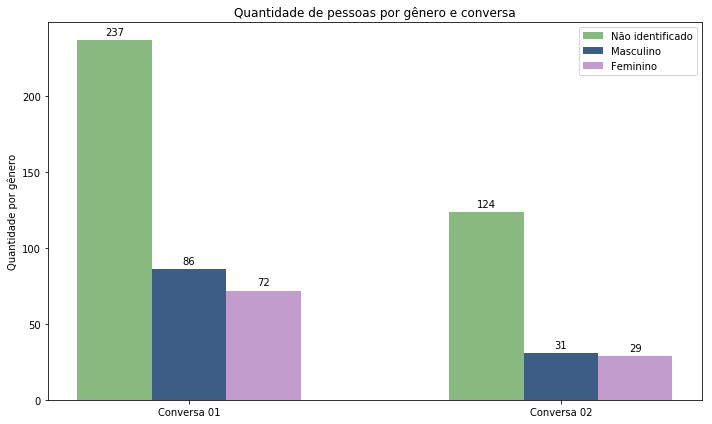
\includegraphics[keepaspectratio=true,scale=0.5]{figuras/tcc2/genero_por_conversa.png}
	\caption{Distribuição de gênero por conversa}
	\label{fig:genero-por-conversa}
\end{figure}

Agrupados por usuários e as somas de seus respectivos votos, pôde-se calcular a porcentagem de votos que discordaram, passaram ou concordaram. 
Uma \textit{feature} binária foi criada para identificar usuários que escreveram algum comentário na mesma conversa. Entretanto, essa \textit{feature} não teve impacto na análise de correlação com os votos como mostra as Fig. \ref{fig:corr-por-usuarios-1} e \ref{fig:corr-por-usuarios-2}.

%Entretanto, os resultados não demonstraram  após as análises e correlações 

Em busca da maior compreensão dos dados, calculou-se a correlação de Pearson $(r)$ para cada conversa nas Fig. \ref{fig:corr-por-usuarios-1} e \ref{fig:corr-por-usuarios-2}. Estas correlações são calculadas em pares de colunas, excluindo valores 
nulos \footnote{\href{https://pandas.pydata.org/pandas-docs/stable/reference/api/pandas.DataFrame.corr.html}{https://pandas.pydata.org/pandas-docs/stable/reference/api/pandas.DataFrame.corr.html}}, ou seja cada coluna será analisada com todas as outras. 

Algumas \textit{features} foram criadas e ao invés de utilizar os dados das somatórias dos votos, foi calculado as porcentagens desses votos. 
Sendo assim estes valores estariam em uma mesma escala $V_{percentage}=[0,1]$. 
Também todos os dados passaram por uma normalização usando o \textit{Z-score} \footnote{\href{https://scikit-learn.org/stable/modules/generated/sklearn.preprocessing.StandardScaler.html\#sklearn.preprocessing.StandardScaler}{Sklearn preprocessing StandardScaler}}
%\footnote{\url{https://scikit-learn.org/stable/modules/generated/sklearn.preprocessing.StandardScaler.html#sklearn.preprocessing.StandardScaler}}. 
Segue as colunas analisadas:

\begin{itemize}
\item total de comentários votados por usuário
\item gênero
\item porcentagem de votos que concordaram
\item porcentagem de votos que passaram
\item porcentagem de votos que discordaram
\item porcentagem de votos não vistos
\item se o usuário criou algum comentário
\end{itemize}

Foi utilizado o coeficiente de correlação Pearson ($r$) que varia entre $-1$ e $1$ e o sinal indica direção positiva ou negativa. Uma correlação perfeita $(-1$ ou $1)$ raramente é encontrado na prática e significa uma relação linear perfeita entre duas variáveis com derivada positiva $(r=1)$ ou negativa $(r=-1)$. A correlação quando for $0$ indica que não há relação linear entre as variáveis \cite{filho2009}. 


\begin{figure}[!h]
	\centering
	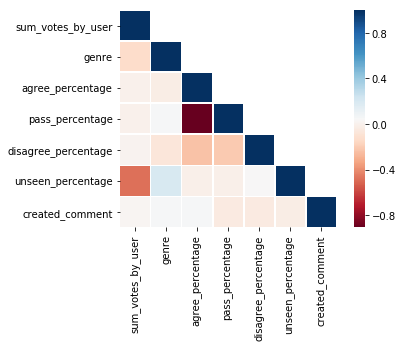
\includegraphics[keepaspectratio=true,scale=0.8]{figuras/tcc2/corr_por_usuarios_1-1.png}
	\caption{Representação da conversa 01 da plataforma EJ}
	\label{fig:corr-por-usuarios-1}
\end{figure}

Na Fig. \ref{fig:corr-por-usuarios-1} a correlação mais forte e também negativa acontece entre a porcentagem de votos que concordam e a porcentagem de votos que passam, com  $r=-0,90$. É esperado uma correlação entre os votos por se encontrarem na mesma escala de porcentagem e é natural o comportamento inverso, por exemplo com o aumento da porcentagem de votos que concordam naturalmente a porcentagem dos demais votos diminuem.

%O que justifica por exemplo, com o aumento da porcentagem de votos que concordam naturalmente a porcentagem dos demais votos diminuem. Essa correlação está muito próxima de perfeita e também inversa, o que pode significar que os participantes concordam muito ou passam muitos os comentários. Existe a correlação com os votos que discordam que é fraca, assim como a minoria dos votos.  %Essa correlação é forte e negativa.% e próxima a correlação perfeita.
%, e traz a relação de que o usuário tende a votar mais ou comentários que concorde ou que passe.
A relação de votos não vistos e a soma de votos tem $r=-0,47$, uma correlação média e negativa. Era esperado a existência de correlação entre essas duas variáveis, pois o usuário vota apenas quando tem acesso aos comentários.
%, de quanto maior a soma dos votos por usuário, menor a chance de ele não ter visto mais comentários. O que seria esperado, pois se o usuário não respondeu 

%Não se pode afirmar 

Na conversa 02 como mostrado na Fig. \ref{fig:corr-por-usuarios-2} os maiores coeficientes de correlação Pearson $(r)$ são as mesmas variáveis da Conversa 01. A porcentagem de votos que concordam e passam, com $r=-0,90$ e a porcentagem de comentários não vistos e a somatória de votos totais com $r=-0,47$. Note que a correlação alta é esperada nestas variáveis pois existe uma dependência linear (ainda que imperfeita) dada pela equação $agree_{percentage} + pass_{percentage} + disagree_{percentage} = 1$. Se $disagree_{percentage}$ for muito baixo, como observado, a correlação tenderia a $-1$. Os dados atuais reforçam a observação de que os usuários votaram mais ou em comentários que concorde ou que passe.


\begin{figure}[!h]
	\centering
	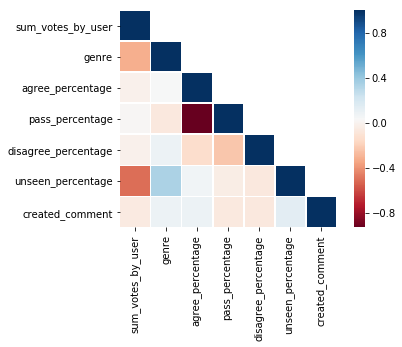
\includegraphics[keepaspectratio=true,scale=0.8]{figuras/tcc2/corr_por_usuarios_2.png}
	\caption{Representação da conversa 02 da plataforma EJ}
	\label{fig:corr-por-usuarios-2}
\end{figure}


O coeficiente  de correlação de Pearson não diferencia entre variáveis dependentes e independentes, ou seja, o valor da correlação entre $X$ e $Y$ é o mesmo entre $Y$ e $X$. A causa não está relacionado com a correlação, ou seja, dificilmente pode-se afirmar quem varia em função de quem. Pode-se dizer que existe semelhanças entre a distribuição dos escores das variáveis \cite{filho2009}.


\subsection{Nuvem de palavras}

%Os comentários foram estudados com o objetivo de entender padrões nos comentários e polarização política. 
%Com o apoio da biblioteca Wordcloud %\footnote{https://amueller.github.io/word_cloud/}.

Todos os comentários foram tratados com a remoção de pontuações e \textit{stopwords}, que são palavras muito comuns que possuem pouco significado como preposições, artigos e conjunções. Depois foram calculados as frequências de cada palavra utilizada nos comentários, valor esse que está diretamente relacionado com o tamanho das palavras na nuvem de palavras. Na Fig. \ref{fig:nuvem-palavras-conversa-1} a nuvem de palavras corresponde à Conversa 01 e na Fig. \ref{fig:nuvem-palavras-conversa-2} corresponde à Conversa 02.


%Com a frequência das palavras em todos os comentários de cada conversa foi possível criar uma nuvem de palavras, onde o tamanho está diretamente relacionado com a quantidade de vezes que foi citado. Então quão maior a palavra, mais apareceu entre os comentários.
%As frases tiveram \textit{stopwords} e pontuações tratadas. Na Figura \ref{fig:nuvem-palavras-conversa-1} a nuvem de palavras corresponde à Conversa 01 e na Figura \ref{fig:nuvem-palavras-conversa-2} corresponde à Conversa 02.


\begin{figure}[!h]
	\centering
	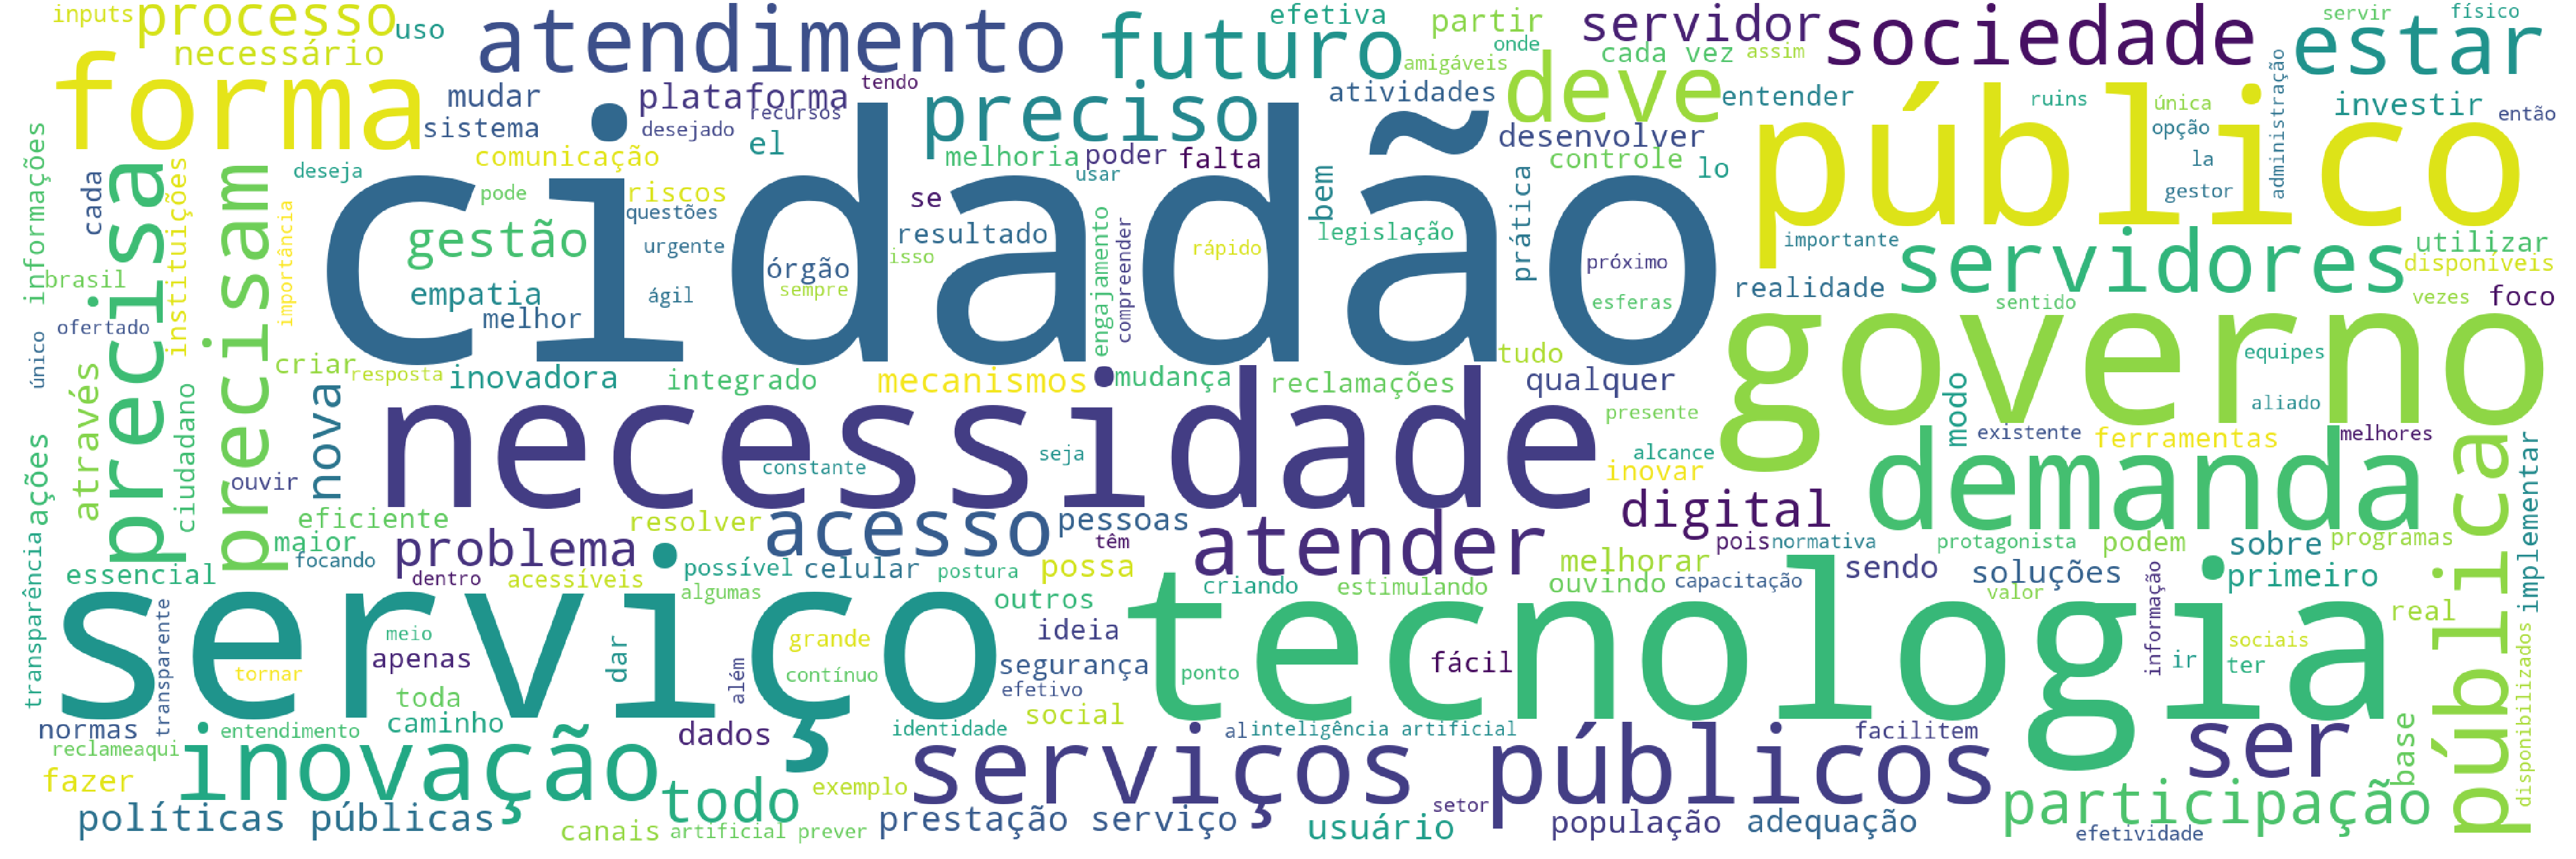
\includegraphics[keepaspectratio=true,scale=0.1]{figuras/tcc2/nuvem/nuvem_palavras_conversa_1.png}
	\caption{Nuvem de palavras da Conversa 01: Como os serviços públicos podem se adequar às demandas do
cidadão do futuro?}
	\label{fig:nuvem-palavras-conversa-1}
\end{figure}


A biblioteca utilizada para a realização das nuvens de palavras faz análise de unigramas e bigramas, ou seja, a frequência de palavras únicas e a ocorrência de duas palavras adjacentes. Em ambas as conversas é possível identificar que existe um padrão de palavras semelhantes, como as palavras mais frequentes cidadão, serviço e governo. 


\begin{figure}[!h]
	\centering
	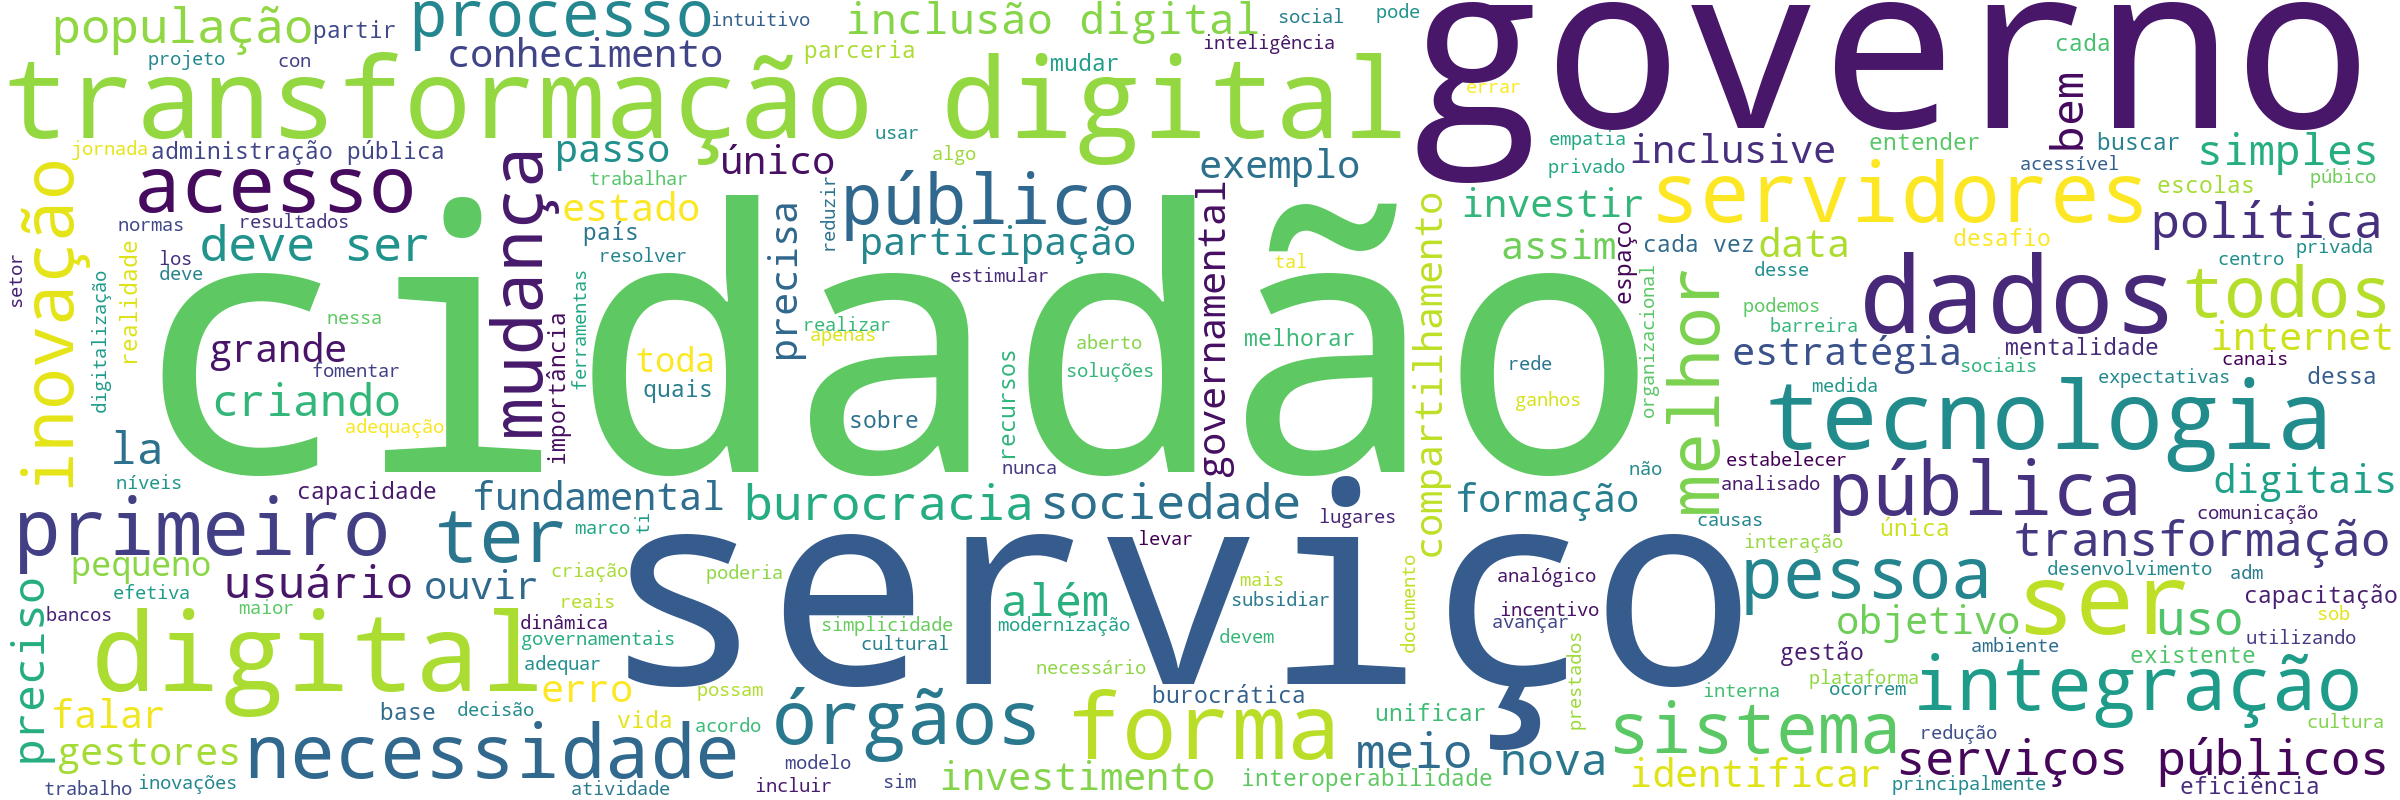
\includegraphics[keepaspectratio=true,scale=0.18]{figuras/tcc2/nuvem/nuvem_palavras_conversa_2.png}
	\caption{Nuvem de palavras da Conversa 02: O que pode ser feito para superar os desafios da  transformação digital do governo?}
	\label{fig:nuvem-palavras-conversa-2}
\end{figure}

Não é possível fazer maiores observações apenas com a frequência das palavras e neste tipo de análise a semântica não é incluída, já que as palavras podem ter distintos significados dependendo da conjuntura gramatical e do contexto. No entanto, a nuvem de palavras é útil para delinear o tópico de conversação.
%A nuvem de palavras é útil, no entanto para delinear o tópico de conversação.
%Entretanto, este conhecimento é válido para
%é um primeiro passo o resultado 
%traz neste primeiro momento o conhecimento
%dessas palavras mais frequentes para cada conversa.


\section{Classificação de perfis de opinião}

\subsection{Comentários}

Muitos comentários não foram visualizados pelos usuários, na qual aproximadamente $40\%$ dos participantes votaram um total de até $5$ comentários.  Logo, para a análise teve de se considerar mais uma opção, comentários não visualizados, totalizando quatro categorias possíveis para cada comentário:

\begin{itemize}
\item Concordar
\item Discordar
\item Passar
\item Não visualizado
\end{itemize}


Para cada conversa é possível ter $n$ comentários, e  cada comentário pode ter apenas uma categoria de voto.
Cada voto possui uma representação númerica para ser utilizado nos modelos de aprendizado de máquina, como pode ser visto na Fig. \ref{fig:fluxo-votos-comentarios}. Entretanto, para a escolha do valor de comentários não visualizados, a fim de que não se influencie em uma escala de grandeza maior ou menor que os valores já escolhidos e também diferenciar da escolha de passar, foi escolhido utilizar a média dos votos.





\begin{figure}[!h]
	\centering
	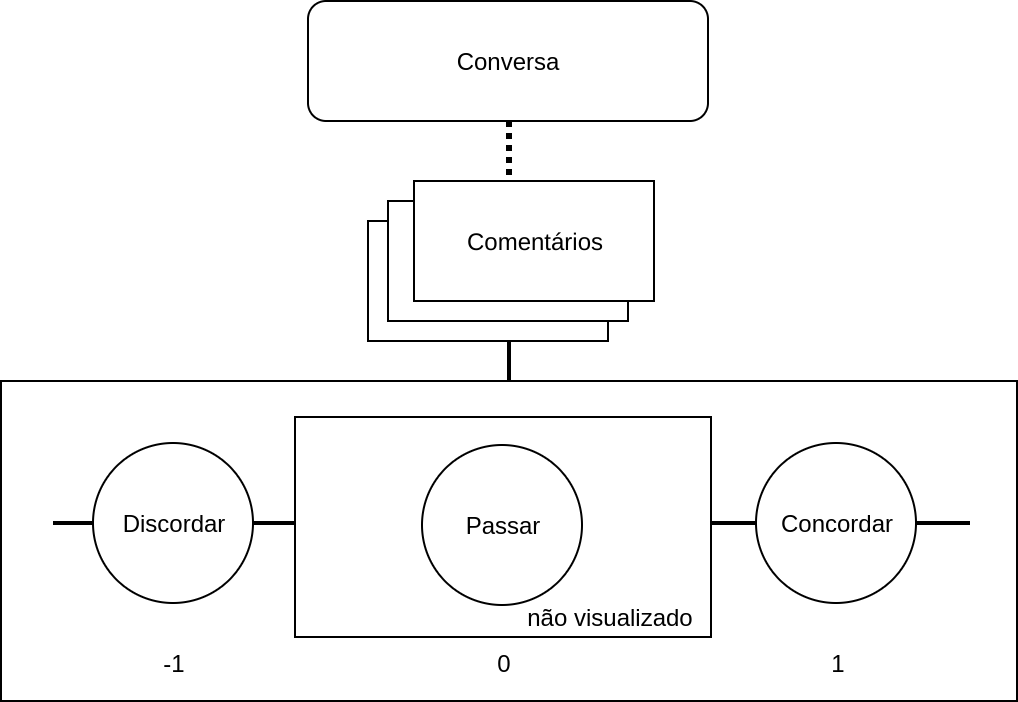
\includegraphics[keepaspectratio=true,scale=0.30]{figuras/tcc2/fluxograma_votos_comentarios.png}
	\caption{Representação de uma conversa da plataforma EJ}
	\label{fig:fluxo-votos-comentarios}
\end{figure}

As categorias de votos podem ser 
%$V=\{v_{-1}, v_{0}, v_{1}, v_{\overline{C_{n}}}\}$, 
$V=\{-1, 0, 1, \overline{C_{n}}\}$
onde $C_{n}$ representa o conjunto de votos para cada comentário $n$.
A quantidade máxima de votos considerada para todos os comentários feitos na conversa é o mesmo que o número de usuários únicos por cada conversa $m$,
%O voto que discorda do comentário é representado por $v_{-1} = -1$, o voto que passa o comentário $v_{0}=0$ e o voto que concorda com o comentário $v_{1}=1$. 

%Cada $C_{n}$ possui $u$ votos, do qual $u$ também representa o número de usuários únicos naquela conversa.

%, e cada comentário é representado por $C_{n} = [c_0, c_1 $

\begin{equation}
{C_{n}} = [v_0, v_1, \dots, v_m], 
\end{equation}

\noindent
e a categoria de votos não visualizados que é representado por $\overline{C_{n}}$, equivale a média dos votos por cada comentário

\begin{equation}
\overline{C_{n}} =  \frac{\sum C_{n}}{n}.
\end{equation}

%v_{\overline{C_{n}}} = \sum \frac{C_{n}}{n}

%O usuário que mais respondeu foi da Conversa 01, totalizando $109$ comentários, ou seja $98\%$.

\subsection{Clusterização}
%% PCA E KMEANS

A fim de identificar grupos de opinião nas conversas, assumimos $k=4$ \textit{clusters} com base nos votos dos usuários em cada comentário. Nessa matriz de comentários por usuários foi utilizado a redução de dimensionalidade PCA e para a classificação de perfis de opinião foi utilizado o modelo não supervisionado \textit{k-means}. O PCA reduziu o conjunto de dimensões de todos os comentários para $2$ componentes principais, que possibilita a visualização em 2D. 

%foi reduzido para dimensão $2$ para

% Neste trabalho assume-se a existência de $4$ perfis de opinião.
%Com a categoria de votos não visualizados sendo $2$ foi possível observar o comportamentos dos \textit{clusters} 

Na Fig. \ref{fig:k-means-conversas} é possível observar o comportamento dos \textit{clusters} nas duas conversas onde cada ponto preto significa o centro de cada agrupamento. Com $\overline{C_{n}} = média\;dos\;votos$, o valor pode transitar entre $-1$ e $1$. Foram incluídos nesta análise comentários que tiveram pelo menos $50$ votos.

\begin{figure}[!h]
	\centering
	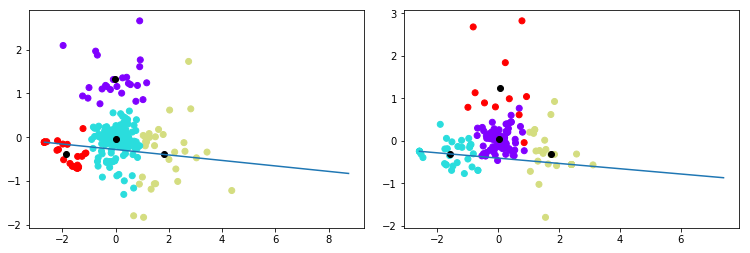
\includegraphics[keepaspectratio=true,scale=0.6]{figuras/tcc2/compara-pca-n50.png}
	%pca_n50_conversa_1
	\caption{K-means aplicado aos comentários com mais de 50 votos - Conversa 01 imagem da esquerda e Conversa 02 imagem da direita }
	\label{fig:k-means-conversas}
\end{figure}



 %comportamento diferente de $v_{\overline{C_{n}}} = média$, como pode ser visto nas Figuras \ref{fig:k-means-2-conversa-1} e 
%na primeira tentativa com o voto não visto sendo $2$.



Os perfis identificados na Conversa 01 estão na direita da Fig. \ref{fig:k-means-conversas} e à esquerda os perfis da Conversa 02.
%na Figura \ref{fig:k-means-50-conversa-2}.
As linhas que aparecem nas imagens 
% da esquerda e direita na Figura \ref{fig:k-means-conversas} 
representam os comportamento extremos. Na extremidade esquerda o usuário concorda com todos os comentários e na extremidade esquerda discorda com todos os comentários.



%\begin{figure}[!h]
%	\centering
	%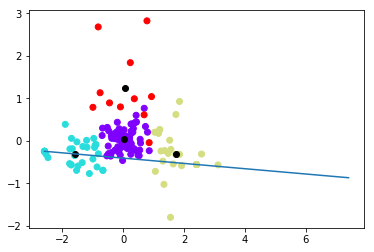
\includegraphics[keepaspectratio=true,scale=0.70]{figuras/tcc2/pca_n50_conversa_2.png}
%	\caption{Conversa 02 - K-means aplicado aos comentários com mais de 50 votos}
%	\label{fig:k-means-50-conversa-2}
%\end{figure}


As linhas das figuras passam bem próximas de três agrupamentos, entre um usuário com total participação e concordância e um usuário com total participação e discordância dos comentários. Era esperado a identificação de grupos de opinião, entretanto, não se pode afirmar a classificação de perfis de opinião nesse momento e sim de concordância.
%Bem próximo as linhas têm 



%Com $v_{\overline{C_{n}}} = média\;dos\;votos$, o valor pode transitar entre $-1$ e $1$, e como 

%Na imagem à esquerda  $v_{unseen}=2$. Na imagem à direita $v_{unsee}=\overline{com_{n}}$}

% Na imagem à esquerda a categoria de votos não visualizados é 2 e na imagem à direita a média dos votos de cada comentário.




%\begin{figure}[!h]
%	\centering
%	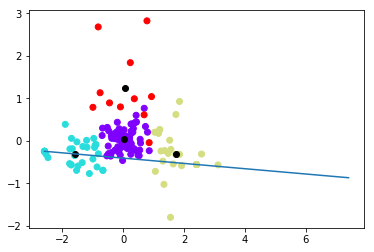
\includegraphics[keepaspectratio=true,scale=0.70]{figuras/tcc2/pca_n50_conversa_2.png}
%	\caption{Conversa 02 - K-means aplicado aos comentários com mais de 50 votos}
%	\label{fig:k-means-50-conversa-2}
%\end{figure}


\subsubsection{Coeficiente de Silhouette}

Foi assumido o valor de \textit{clusters} como $k=4$, entretanto, com apoio de métricas foi calculado o Coeficiente de Silhouette para validar essa escolha inicial. Foi utilizado os valores de $k=[2,3,4,5]$ nas duas conversas como mostra a Tab. \ref{tab:silhouette-usuarios}. 

\begin{table}[!h]
\centering
\label{tab:silhouette-usuarios} 
\begin{tabular}{|c|c|c|}
\hline
    & \textbf{Conversa 01} & \textbf{Conversa 02} \\ \hline
k=2 & 0.4422               & 0.3231               \\ \hline
k=3 & 0.2826               & 0.2386               \\ \hline
k=4 & 0.1892               & 0.2195               \\ \hline
k=5 & 0.1783               & 0.2412               \\ \hline
\end{tabular}
\caption{Coeficiente de Silhouette - Clusterização dos votos dos usuários}
\end{table}


Lembrando que os valores do coeficiente apenas auxiliam a escolha das categorias, para uma definição mais concreta é preciso mais análises. De acordo o cálculo do Coeficiente de Silhouette, quão mais próximo de $1$ melhor o resultado dos agrupamentos e os 	valores próximos a $0$ indicam \textit{clusters} sobrepostos. 


Nas Fig. \ref{fig:compara-cluster-conversa1} e \ref{fig:compara-cluster-conversa2} temos a clusterização da Conversa 01 e da Conversa 02 com os diferentes valores de $k$. 

Na Conversa 01, os melhores valores foram atribuidos à $k=2$ e $k=3$, o que levanta questionamentos sobre a escolha inicial. O valor de $k=2$ não será considerado para ambas as conversas, mesmo com valores maiores, pois como já dito anteriormente, o coeficiente traz mais uma informação e não necessariamente só ele seja suficiente. E foi observado durante esse estudo que a escolha $k-2$ geralmente traz resultados melhores, entretanto, pode existir outros \textit{clusters} dentro de algum. Quando se tem uma escolha tão pequena de \textit{clusters}, pode ser que outros estejam sobrepostos, por isso a necessidade de verificar outros valores e escolher o que faz mais sentido para o contexto.


\begin{figure}[!h]
	\centering
	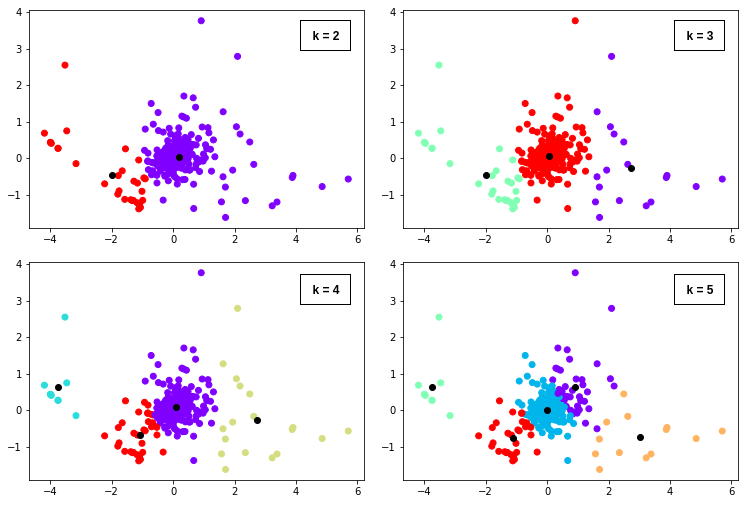
\includegraphics[keepaspectratio=true,scale=0.58]{figuras/tcc2/compara-k-clusters-conversa-1.png}
	%pca_n50_conversa_1
	\caption{K-means com $k=[2,3,4,5]$ na Conversa 01}
	\label{fig:compara-cluster-conversa1}
\end{figure}

Logo na Conversa 01, o valor mais interessante neste momento com base no Coeficiente Silhouette, nas análises e no comportamento dos \textit{clusters}, $k=3$, talvez seja uma escolha interessante nesse momento e com os dados atuais.


\begin{figure}[!h]
	\centering
	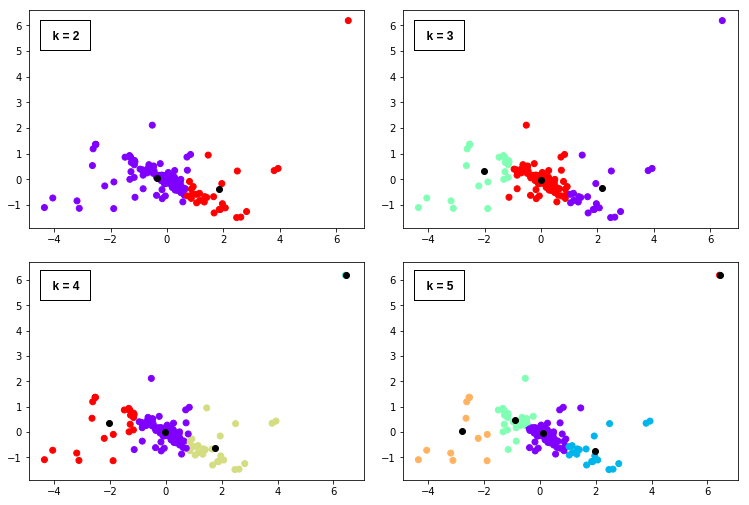
\includegraphics[keepaspectratio=true,scale=0.58]{figuras/tcc2/compara-k-clusters-conversa-2.png}
	%pca_n50_conversa_1
	\caption{K-means com $k=[2,3,4,5]$ na Conversa 02}
	\label{fig:compara-cluster-conversa2}
\end{figure}
%compara-k-clusters-conversa-2


Na Conversa 02, também não será considerado nesse momento o valor de $k=2$. Outros melhores valores foram de $k=5$ e $k=3$, respectivamente, e com base nessas informações e em todas as análises $k=3$ seria uma boa escolha de \textit{clusters} para esta conversa. Podemos perceber que existem alguns dados no canto superior esquerdo nas imagens que em $k=[4,5]$ se tornam \textit{clusters} isolados. Estes dados talvez sejam apenas \textit{outliers}, ou seja, um valor atípico que apresenta bem distante dos demais dados e que geralmente causam prejuízo a interpretação dos resultados. 


%É importante ressaltar a necessidade de maior quantidade de dados.


\section{Clusterização por comentários}

A clusterização dos comentários com base nas \textit{features} tem a intenção de identificar comentários semelhantes e correlações que auxiliem o comportamento dos votos.

Os comentários foram agrupados em busca de uma maior compreensão dos dados. Os dados mais relevantes dos comentários para este trabalho são os conteúdos dos comentários, quantidade dos votos e data de aprovação. A partir desses dados foi possível criar outras \textit{features} para o estudo. As features criadas foram:
%criador do comentário e datas de criação, modificação
%Para essa análise foram organizadas e criadas \textit{features} 

%Para a \textit{features} de maiores relevância e que retiram 


\begin{itemize}
\item porcentagem de votos que concordaram
\item porcentagem de votos que passaram
\item porcentagem de votos que discordaram 
\item votos totais por comentário
\item data de atualização do comentário
\item tamanho do comentário
\item média de palavras por comentário

\end{itemize}



É esperado que exista correlação entre o tamanho do comentário e a porcentagem de votos pulados, o que refletiria possivelmente o comportamento dos usuários desistirem de ler os comentários devido ao tamanho. Entretanto na Fig. \ref{fig:compara-corr-comentarios} a correlação praticamente não existe. 

\begin{figure}[!h]
	\centering
	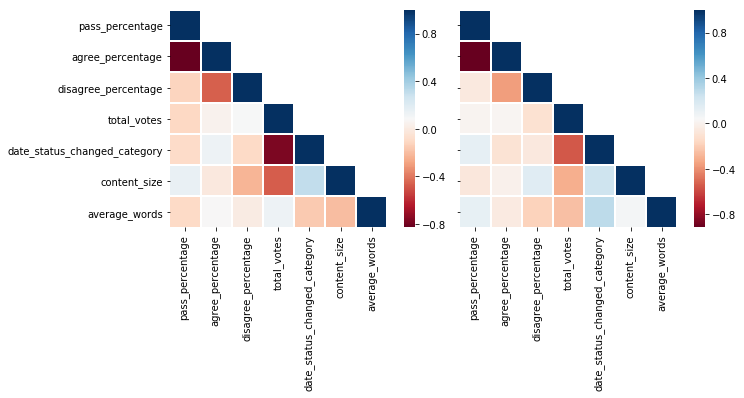
\includegraphics[keepaspectratio=true,scale=0.58]{figuras/tcc2/cluster-comentario/corr-comentario-conversa2.png}
	%pca_n50_conversa_1
	\caption{Correlação aplicado aos comentários - Conversa 01 ao lado esquerdo e Conversa 02 ao lado direito}
	\label{fig:compara-corr-comentarios}
\end{figure}

O tamanho do comentário possui correlação média $r=-0,46$ com total de votos na Conversa 01 (à esquerda) da Fig. \ref{fig:compara-corr-comentarios}.

%as desistência de lerem os comentários.
A data de aprovação do comentário tem correlações de $r=-0,77$ e $r=-0.55$ respectivamente nas Conversas 01 e 02, 
%Também a data de aprovação do comentário esteja relacionado a quantidade de votos, 
o que pode evidenciar a ordem atual, possivelmente data de aprovação crescente, que os comentários chegam a cada usuário.


\begin{figure}[!h]
	\centering
	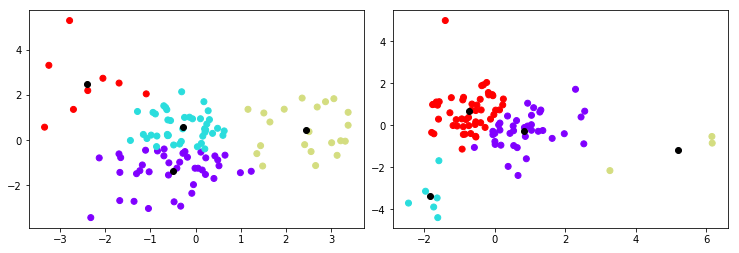
\includegraphics[keepaspectratio=true,scale=0.6]{figuras/tcc2/cluster-comentario/compara-comentarios.png}
	%pca_n50_conversa_1
	\caption{Conversa 01 à esquerda e Conversa 02 à direita - K-means aplicado aos comentários}
	\label{fig:k-means-comentario-conversas}
\end{figure}


As colunas de votos foram transformadas em colunas de porcentagem dos votos. É esperada uma correlação alta e negativamente linear entre as porcentagens de passar e aceitar. Os valores foram $r=-0.82$ e $r=-0.91$, já que existe uma relação linear $aprovar = 1 - discordar + pular$.

% todavia essa dependência linear é explicada em \ref{chap:dados-reais}.
%A correlação confirma esses valores com $r=-0.82$ e $r=-0.91$. 

%A alta correlação entre as porcentagens de votos que concordam e passam 

%A data de aprovação do comentário e o total de votos tem correlação média, entretanto não se obteve resultado relevante sobre a porcentagem de votos pulados e o tamanho do texto.

%entretanto não se obteve resultado relevante sobre a porcentagem de votos pulados e o tamanho do texto.

Na Fig. \ref{fig:k-means-comentario-conversas} temos o agrupamento dos comentários das duas conversas. O número de comentários é menor que o de usuários, o que implica na redução de dados também para análise. Na Conversa 01, imagem à esquerda, os dados se encontram mais dispersos e dois \textit{clusters} bem próximos. Já na Conversa 02, imagem à direita, dois \textit{clusters} estão bem próximos e abrange grande parte dos dados, deixando $2$ \textit{clusters} mais distantes em extremos. 

%Nessa clusterização foi utilizada a métrica do 
O Coeficiente de Silhouette foi aplicado como uma métrica de apoio, para comparar a escolha do $k=4$ e as observações feitas quanto a distribuição dos dados. Então foi calculado o coeficiente para $k=[2,3,4,5]$ que resultou a Tab. \ref{tab:silhouette}. 


\begin{table}[!h]
\centering
\label{tab:silhouette} 
\begin{tabular}{|c|c|c|}
\hline
    & \textbf{Conversa 01} & \textbf{Conversa 02} \\ \hline
k=2 & 0.2567               & 0.2041               \\ \hline
k=3 & 0.2379               & 0.2372               \\ \hline
k=4 & 0.2415               & 0.2291               \\ \hline
k=5 & 0.2126               & 0.2071               \\ \hline
\end{tabular}
\caption{Coeficiente de Silhouette - Clusterização por comentários}
\end{table}

Os valores variam entre $[-1,1]$, e o melhor valor para o coeficiente é $1$. Os valores estão bem próximos, como pode ser visto na Tab. \ref{tab:silhouette}. Na Conversa 01, a escolha de $k=4$ mostrou um bom resultado, considerando que $k=2$ não seja uma escolha e foi calculado por fins de comparação. Na Conversa 02, o melhor valor foi de $k=3$ e reforça a observação feita sobre a proximidade dos dois \textit{clusters}.


\chapter{Conclusão}
\label{chap:conclusao}

%Era esperado
%No primeiro momento 

Com os dados do EJ era esperado algum tipo de correlação entre o tamanho do comentário e a porcentagem de votos, mas não se obteve nada substancial. 
A data de aprovação dos comentários é o dia em que o comentário passou a estar visível para os usuários. Era esperado a correlação desta data com a soma de votos por comentário, talvez porque os comentários apareçam por ordem de aprovação, ou seja, os comentários que foram criados primeiro também aparecerão primeiro. Essa correlação negativa existe e uma recomendação seria que a plataforma implementasse algum tipo de estratégia que favoreça os comentários com menos votos. 

A base de usuários possuía identificadores iguais para pessoas diferentes nas duas conversas, uma sugestão seria a padronização desses identificadores até para avaliar se um mesmo usuário participou de mais de uma conversa. Realizada a clusterização dos participantes das conversas, não podemos concluir a classificação dos perfis de opinião, mas o nível de concordância. 


Foi assumido no início deste trabalho $k=4$ \textit{clusters} de perfis de opinião, entretanto, com os dados trabalhados e após todas as análises a melhor escolha desse valor é $k=3$. Reforçando que este não é um valor que necessariamente funcionará com todos os dados da plataforma. Se faz uma boa escolha perante todo o estudo.
%e por isso a importância de mais dados e análises 


A maioria dos votos concordaram com os comentários, reforçando a hipótese levantada desde a criação dos dados sintéticos e que pode estar relacionada as pessoas criarem comentários que tenha uma alta aceitação, e a análise semântica pode contribuir nesse entendimento e na formação de opiniões. Assim como conversas ou comentários que incluam temas que gerem maior discussão.


% dos comentários e de conversas que facilitam a polarização dos participantes. 

%O objetivo de if
%Desta forma equilibrando a média de votos por comentário e  de forma a equilibrar os votos

%Com a clusterização dos participantes das conversas ainda não podemos concluir a classificação dos perfis de opinião, mas o nível de concordância é um primeiro passo. 

%A experiência de trabalhar com os dados reais torna o impacto deste estudo ainda maior, entretanto, os obstáculos de lidar com um cenário diferente do mundo ideal atrasou a finalização e a não execução de um dos objetivos dos modelos descritivos 
% não trouxe nesse momento 

%Para a conclusão dos objetivos específicos, 

A experiência de trabalhar com os dados reais torna o impacto deste estudo ainda maior, e mesmo com os obstáculos contornados ainda tem muito trabalho a ser feito, principalmente pela importância e impacto que o Empurrando Juntos traz a sociedade.

%entretanto, os obstáculos de lidar com um cenário diferente do mundo ideal 

Em síntese, para trabalhos futuros, é sugerida estruturação e maior quantidade de dados reais, incluindo dados de conversas, usuários e comentários. Os dados que caracterizam os usuários como gênero, idade e localidade acrescentam na formação dos grupos de opinião. É de suma importância a qualidade destes resultados para a visualização das bolhas de opinião na plataforma.

 


%das identificação dos grupos 
%Analisar os comentários semanticamente também auxilie no entendimento de comentários similiares e comentários que facilitem a polarização de usuários. 


%A clusterização dos comentários


%O desenvolvimento e a continuação deste trabalho traz informações e transparência para a sociedade e 
%Para trabalhos futuros é importante a maior quantidade de dados para as análises, a análise semântica dos comentários. 

%Em síntese dos



%Os modelos estatísticos 




%A importância de plataformas participativas que 

%EJ softer livre , contribuição


%O desenvolvimento deste trabalho ag






%Por meio da execução deste trabalho, foi possível perceber a variação dos algoritmos e modelos em um cenário onde os usuários possuem apenas as opções de concordar e discordar de comentários. O que não reflete ainda a realidade, pois existe também a opção de pular um comentário e não ter visualizado. Os dados utilizados como insumos são os usuários e os votos dos comentários para a classificação de perfis.

%Este primeiro momento foi trabalhado os modelos estatísticos e os algoritmos ainda em um cenário ideal, a continuidade dele se dará por meio do estudo dos algoritmos \textit{k-means} e \textit{k-means} modificado, este último utilizado no EJ atualmente. Também abrangindo as demais opções de um usuário real. Segue o cronograma na Tab. \ref{tab:cronograma}:

%No Naive Bayes todos os comentários são considerados independentes e tende a convergir ao máximo de acerto (votos certos/ votos totais). A variação de parâmetros como a quantidade de votos por usuário e dos $\alpha$s podem influenciar no atraso do resultado.



%A continuidade do trabalho incluirá o estudo dos algoritmos \textit{k-means} e \textit{k-means} modificado. Este último utilizado no EJ atualmente. Segue o cronograma na Tab. \ref{tab:cronograma}: %Além do acréscimo das opções pular, 

%Além da proximidade com o  acréscimo das opções 

% Please add the following required packages to your document preamble:
% \usepackage[table,xcdraw]{xcolor}
% If you use beamer only pass "xcolor=table" option, i.e. \documentclass[xcolor=table]{beamer}




